\documentclass[conference]{IEEEtran}
\IEEEoverridecommandlockouts
% The preceding line is only needed to identify funding in the first footnote. If that is unneeded, please comment it out.
%Template version as of 6/27/2024

\usepackage{cite}
\usepackage{amsmath,amssymb,amsfonts}
\usepackage{algorithmic}
\usepackage{graphicx}
\usepackage{textcomp}
\usepackage{xcolor}
\usepackage{float} 
\usepackage{tabularx} 
\usepackage{appendix} % Added for appendix support

\def\BibTeX{{\rm B\kern-.05em{\sc i\kern-.025em b}\kern-.08em
    T\kern-.1667em\lower.7ex\hbox{E}\kern-.125emX}}
\begin{document}

\title{Smart Plans, Smarter Choices: Enhancing Mobile Data Selection with Chatbots}

\author{\IEEEauthorblockN{David Carciente - 40247907}
\IEEEauthorblockA{\textit{Concordia University} \\
Montreal, Canada \\
davidcarciente@outlook.com}
\and
\IEEEauthorblockN{Brian Tkatch - 40191139}
\IEEEauthorblockA{\textit{Concordia University} \\
Montreal, Canada \\
brian@briantkatch.com}
}

\maketitle

\begin{abstract}
This paper investigates the persistent mismatch between consumers' actual mobile data needs and their plan selections, which frequently leads to overspending and frustration. We propose an intelligent deterministic chatbot solution that analyzes individual usage patterns and translates complex pricing structures into understandable recommendations through natural language interaction. By addressing the cognitive barriers documented in telecommunications research, our approach bridges the gap between technical specifications and real-world usage goals, empowering users to make confident, informed decisions when selecting mobile data plans. The solution directly targets the psychological factors that currently drive suboptimal consumer choices, offering both users and providers a more efficient path to appropriate plan selection.
\end{abstract}

\section{Introduction}
The internet is continuously expanding with numerous services that help humans accomplish their daily tasks and fulfill various needs. However, accessing the internet from anywhere and at any time comes at a cost. Recognizing that individuals have varying data requirements; telecommunication companies typically offer multiple tiers of bandwidth. This means not all users require access to the same amount of data.
Given these varying needs, telecommunication companies present different plans, often summarized in feature matrices. These matrices provide high-level details, such as bandwidth, speed, and cost. However, there's often no clear correlation between these attributes and actual user usage, leading to confusion. This raises an important question:
\begin{quote}
How much data does a user genuinely need to accomplish their daily goals on the internet?
\end{quote}

\subsection{Hypothesis}

Ensuring mobile phone plans accurately align with users' actual data needs is essential for a positive purchasing experience. Mismatched plans, where users pay for too much or too little data, often lead to dissatisfaction. This paper hypothesizes that an onboarding chatbot can effectively gather user insights, bridging the gap between users' real data requirements and the available plans, thus recommending the optimal data plan.

\subsection{Objectives, Motivations, Theoretical Contribution Goals, and Target Audience}

The primary objective of this paper is to investigate current barriers users face when interacting with telecommunication services to purchase mobile phone plans. This research is motivated by extensive evidence showing that consumers frequently make suboptimal choices when selecting mobile plans \cite{b3}, \cite{b1}, leading to significant overspending due to both underusing and overusing plan allowances. Studies indicate that 21\% of consumers choose overly large plans while 18\% select inadequate ones \cite{b3}, suggesting a systematic market inefficiency that merits investigation. This recurring mismatch indicates an unmet need for clearer, more intuitive guidance during plan selection processes.

From a theoretical perspective, this work will contribute to understanding how salience bias \cite{b3} and bounded rationality \cite{b1} affect consumer decision-making in complex pricing environments. The research will explore how information presentation and decision support tools can mitigate cognitive biases that lead to poor plan selection.

The proposed chatbot solution will be situated within the design space of intelligent decision support systems, exploring the tension between automation and user agency, and between personalization and privacy. Key design decisions include the level of abstraction in user-system communication, the balance between proactive recommendations and user-initiated queries, and methods for explaining complex tariff structures in intuitive ways.

The target audience includes all users paying for data plans but lacking clarity on their actual data consumption. Ultimately, this approach aims to empower users to confidently select suitable plans without worrying about overpaying or underestimating their data needs.
\subsection{Research Method}
The research method uses the Designs Council's Double Diamond process. This process is an IxD process, which can be broken down into several stages. The first stage is discovering the problem from a user centric point of view. This includes discussing all aspects of users choosing a mobile phone plan. The next stage is narrow down the scope of findings, and establishing links, which are deducted into postulates / requirements. The requirements will be addressed via the research of the Chatbot. Then, potential solutions will be explored. A visualization of this process can be found in Appendix A, Figure~\ref{fig:Design Council's Double Diamond}.

\section{Background / Related Work and Readings}
This section will cover readings related to understanding the problem space, between users and choosing a phone plan. 
\subsection{Phone Plans and Telecommunication}
\subsubsection{Understanding the Choice Environment}
Mobile phone plan selection presents consumers with a highly complex decision environment. Friesen and Earl found that consumers consider this task "exhausting and distressing" \cite{b1}, even more challenging than health insurance or retirement decisions. The complexity stems from multiple simultaneous factors: "consumers face not just a large array of options, but also difficulties in ranking them" \cite{b1} with various usage categories (calls, data, messaging) priced differently. Additional complications include connection fees, on/off-network price differentials, peak/off-peak rates, and variable billing increments from 30-second to 1-second blocks \cite{b1}. This multidimensional complexity creates significant cognitive burden for consumers trying to identify optimal plans.
\subsubsection{Multipart Tariffs}
Multipart tariff structures further complicate phone plan decisions. These pricing schemes involve "a fixed fee [that] buys some 'included value' (typically a multiple of the fee), which can be used on a whole range of included usage categories. On reaching the limit (or 'cap'), overage rates apply" \cite{b1}. Consumers rarely receive clear information about the difference between above-cap and below-cap prices, which "may be tenfold or even more" \cite{b1}. These tariffs with increasing usage costs appear designed to extract consumer surplus, either from those who underestimate usage or by pushing consumers into unnecessarily large monthly commitments to avoid overage charges \cite{b1}. Such pricing structures have led to increased consumer complaints and dissatisfaction with telecommunications providers \cite{b1}.
\subsubsection{Mutual Network Carriers}
Network effects significantly influence mobile phone plan selection. Research shows consumers are willing to pay about 2.5 euros more per month to join a larger carrier network \cite{b2}. Interestingly, customers are twice as sensitive to price changes for calls within their own network compared to calls to other networks \cite{b2}. This means people care more about the cost of calling friends and family on the same carrier as them, even if they don't explicitly say so. This explains why carriers often charge less for "same-network calls" and more for "other-network calls" - it encourages people to join networks where their social connections are already members.
\subsubsection{Limited Consumer Understanding of Mobile Plan Pricing}
Research by Friesen and Earl reveals most consumers struggle to understand mobile phone pricing. Their study showed only 18\% of participants could correctly answer three basic questions about phone plan costs, while 25\% couldn't answer any correctly \cite{b1}. Consumers particularly struggled with understanding "included value" in plans - only 25\% knew how charges work when exceeding their plan's cap, and just 49\% understood how charges apply when staying under the cap. Even calculating a basic phone call cost proved difficult for 40\% of participants. What makes these findings concerning is that all study participants already owned mobile phones, suggesting that even with experience, many consumers can't grasp the pricing structures that determine their bills. This widespread confusion helps explain why people often choose unsuitable plans and experience unexpected high charges.
\subsection{User Interaction Design - Psychological Analysis during the Mobile Phone Plan Selection}
\subsubsection{Cognitive Overload and Complexity}
Friesen and Earl's research demonstrates how cognitive limitations impact consumers' mobile plan choices. Even with only seven plans to choose from in experimental conditions, participants made consistently poor decisions due to bounded rationality when facing complex pricing structures \cite{b1}. Notably, multipart tariffs with included values exceeding monthly fees (creating increasing marginal costs) proved most difficult for consumers to process, leading to the worst decision outcomes. The researchers found that not all complexity affects decision quality equally - simply removing fee structures didn't necessarily improve decisions. Instead, specific pricing structures with two-tier increasing marginal costs created disproportionate cognitive challenges \cite{b1}. This suggests certain types of complexity overwhelm consumers' analytical capabilities, leading to suboptimal choices even among mathematically capable individuals.
\subsubsection{Limited Attention and Heuristic Thinking}
Consumers selecting mobile phone plans often rely on cognitive shortcuts rather than calculating optimal choices due to limited attention \cite{b3}. Jin et al. found that consumers exhibit "salience bias," where decisions are overly influenced by noticeable experiences of either overusing or underusing their plan's allowance. This leads to predictable switching behaviors: those exceeding allowances tend to upgrade plans while those underutilizing downgrade, even when their current plan is actually cost-optimal \cite{b3}. This demonstrates how heuristic thinking shapes consumer decisions when facing complex choices.
\subsubsection{Fear of Overspending}
Consumer anxiety about unexpected charges and bill shock significantly influences mobile plan selection. Jin et al. \cite{b3} demonstrate that this fear drives users to adopt precautionary behaviors, often selecting plans with unnecessarily large allowances as a form of "insurance" against potential overage charges. This explains why approximately 21\% of consumers choose excessively large plans, overspending an average of 11.4 CNY monthly \cite{b3}. Confraria et al. \cite{b2} provide complementary evidence, revealing consumers' willingness to pay premiums (1.3 Euros monthly) to reduce commitment periods, reflecting their fear of being locked into suboptimal arrangements. This anxiety-driven decision-making helps explain why, despite consumers' stated goal of cost minimization, they often make choices that prioritize predictability over actual cost efficiency. The psychological comfort of avoiding unexpected charges appears to outweigh the rational calculation of minimum expected costs.
\subsubsection{Desire for Plan Optimization}
Consumers demonstrate a clear desire to optimize their mobile plan choices and minimize costs, yet often struggle to achieve this goal due to cognitive limitations. As Jin et al. explain, "Although consumers intend to pay less by choosing the cost-minimizing plan, they have limited attention to solve the problem" \cite{b3}. This tension between optimization goals and cognitive constraints creates a fundamental challenge in telecommunications markets. Users want to find the perfect balance—"not too much nor too little"—in their plan selection, but frequently rely on simplistic heuristics rather than comprehensive cost calculations \cite{b3}. The difficulty lies in the cognitive demands of accurately forecasting usage and comparing complex multi-part tariff structures, leading consumers to fall back on more immediately available but potentially misleading signals when making switching decisions.
\subsection{Case Studies - Existing Solutions}
\subsubsection{The Hierarchical Decision Model (HDM) and Process (AHP)}
The HDM and AHP provide a systematic approach to solving the complex problem of smartphone and mobile plan selection \cite{b4}. By breaking down the decision-making process into a hierarchical structure with multiple levels of criteria and sub-criteria, these methods help users navigate the overwhelming array of choices in the mobile telecommunications market \cite{b5}. The primary purpose of these models is to transform a subjective decision into a quantitative framework that allows for a more structured and rational evaluation of alternatives. By incorporating both objective measurements and subjective preferences from decision-makers, HDM and AHP enable a comprehensive assessment of smartphone and tariff plan options, considering factors such as technical specifications, cost, service quality, and customer-specific needs.
\subsubsection{Order Preference by Similarity to Ideal Solutions (TOPSIS), Graph Theory and Matrix Approach (GTMA))}
TOPSIS and GTMA are multi-criteria decision-making techniques that help solve complex mobile plan selection problems. TOPSIS works by finding options closest to an ideal solution and furthest from a negative one, while GTMA represents selection criteria as a graph and uses matrix calculations to rank alternatives \cite{b4}. Chang et al. applied these methods to help taxi service operators choose the optimal smartphone and mobile plan combination, finding that the Lenovo A2016 with the "Optimist Talk" plan best met their needs based on factors like monthly cost, battery life, and talk time \cite{b4}. These techniques are valuable because consumers often struggle to compare complicated phone plans with multiple pricing features, frequently leading to poor choices where they pay too much or select inadequate plans \cite{b1}, \cite{b3}.
\subsubsection{Data Monitoring Tool}
Data monitoring tools represent a promising solution to address the challenge of mobile plan selection. One such system, proposed by Achyuth et al., is a mobile application that tracks users' actual usage patterns, including data consumption, call duration, and SMS frequency over a specified period, and then intelligently suggests optimal prepaid plans that align with these patterns \cite{b6}. This approach directly addresses the cognitive limitations identified by Friesen and Earl \cite{b1}, where consumers struggle to evaluate complex pricing structures and often make suboptimal choices. The application employs a hybrid recommender system that considers multiple factors simultaneously, calculating a "desirability quotient" for each available plan based on the ratio of benefits (data, calls, SMS) to costs, thereby simplifying the decision-making process. Unlike existing recharge applications that merely present lists of available plans, this solution actively analyzes usage data to recommend personalized options, potentially reducing both the "fear of overspending" that drives consumers to select unnecessarily large plans \cite{b3} and the cognitive overload associated with complex pricing structures \cite{b1}. This automated approach to mobile plan selection represents a practical implementation of user-centric design in addressing the documented difficulties consumers face in telecommunications markets.
\subsection{Alternative Perspective - Mobile Plan Provider}
\subsubsection{Exploitation of Consumer Biases}
Mobile telecommunications companies strategically exploit consumer biases through deliberately complex pricing structures. Empirical research identifies this industry as a "confusopoly," where carriers intentionally confuse rather than compete on price \cite{b1}. The exploitation of bounded rationality is evident in multipart tariffs with increasing marginal costs, which experimental studies show lead to the poorest consumer decisions \cite{b1}. When faced with these complex structures, consumers often select suboptimal plans due to salience bias, with 21\% choosing unnecessarily large plans as "insurance" against potential overage charges \cite{b3}. This pricing obfuscation strategy was explicitly acknowledged by former Telecom New Zealand CEO Theresa Gattung, who admitted the industry has "used confusion as its chief marketing tool" \cite{b1}.
\subsubsection{Strategic Pricing}
Mobile phone companies use smart pricing strategies to get the most value from different types of customers. They offer different plans with various features, so people can choose what fits them best—but this also lets companies charge more to those willing to pay. They design the plan options in a way that makes customers lean toward more expensive choices, using something called the "compromise effect"—where people tend to pick the middle option rather than the cheapest or most expensive one \cite{b3}. They also use time-based tactics, like starting with low introductory prices that increase later. Instead of charging for using too much data, they often slow down your speed, making you choose between paying more or dealing with slower service \cite{b1}. Altogether, these strategies help companies earn more while staying competitive, by using common patterns in how people make decisions.
\subsubsection{Laws and Regulations}
Telecommunications regulations extend beyond commitment periods to address broader consumer protection issues in mobile plan selection. Many regulatory bodies worldwide have implemented mandatory disclosure rules requiring standardized plan information formats to reduce cognitive overload \cite{b3}. Some jurisdictions enforce cooling-off periods for telecommunications contracts and require notifications when consumers approach data limits. In markets like Australia and the UK, regulators have mandated usage monitoring tools, directly addressing the information asymmetry that leads to suboptimal plan selection \cite{b6}. These measures acknowledge the psychological factors identified by Friesen and Earl that make mobile plan selection particularly difficult for consumers, especially when facing complex multipart tariffs \cite{b1}.
\section{Postulates for the Users Involved in Mobile Plan Selection}\
Based off the research discussed, the following postulates can be derived to understand the problem space. The left margin traces to one of the articles discussed. Some articles and case studies are not traced, as they are for understandidng the problem space, and will be used during the technical requirements level. 
\subsection{User Requirements (8)}
\begin{enumerate}
\item [{B1, C1}: (1)] The user's decision of a mobile plan should not be stressful or confusing.
\item [{B1, B3}: (2)] The user's mobile plan's service fees should be clearly presented and explained to the user.
\item [{B2}: (3)] The user should be able to select their preferred mobile carrier.
\item [{B3, C3}: (4)] The user should be informed of the data plan in terms of their usability goals in natural language, not just their technical bandwidth.
\item [{B1, C2}: (5)] The user should be informed about the value from the cost of the plan.
\item [{C1, B3}: (6)] The user should be able to be informed about the differences between higher or lower tiered plans.
\item [{B2, C2}: (7)] The user should be able to compare their carrier's plan with other carriers.
\item [{C3, B1}: (8)] The user should use an interface when selecting their phone plan, that follows a standardized format to reduce cognitive overload.
\end{enumerate}

\section{Addressing User Requirements using a Chatbot}
\subsection{What is a Chatbot?}
A chatbot is a software application designed to conduct conversations with human users through text or voice interactions, simulating human-like dialogue within a structured interface to accomplish specific tasks. Deterministic chatbots operate through predefined rules, decision trees, and pattern matching, offering predictable responses and controlled conversation flows that are ideal for scenarios requiring consistent information delivery but limited in handling unexpected queries. In contrast, AI-powered chatbots leverage natural language processing and machine learning algorithms to understand context, learn from interactions, and generate more flexible responses, enabling them to handle a wider range of queries and adapt to user needs but potentially introducing unpredictability in responses. This distinction is particularly relevant when designing mobile plan selection systems, where deterministic approaches offer reliability and testability advantages, while AI-based solutions provide more natural conversations that can better address the cognitive overload issues identified in our research.
\subsubsection{Chatbots in Education}
Chatbots offer a promising solution to overcome digital literacy barriers in educational contexts. Mendoza et al. developed a model specifically designed for less tech-savvy users who found traditional learning systems overwhelming \cite{b7}. Their study revealed that many teachers (over 60\%) described themselves as digitally illiterate, with experience limited to basic internet tasks. The chatbot solution provided a familiar, conversational interface resembling WhatsApp, which both students and teachers could easily navigate. User evaluations showed positive results, with students rating the system particularly highly across all measured dimensions. This approach directly addresses several user requirements, particularly satisfying requirement 1 by reducing stress in the decision process, requirement 4 by presenting information in natural language, and requirement 8 by creating a standardized interface that reduced cognitive overload for users with limited technical expertise.
\subsubsection{Chatbots in E-Commerce}
Chatbots have revolutionized e-commerce by providing interactive, conversational interfaces that efficiently gather customer information. Jain et al. found that users preferred chatbots offering either human-like conversation or engaging experiences within familiar messaging platforms \cite{b8}. Building on this, Illescas-Manzano et al. demonstrated that implementing chatbots via Facebook Messenger significantly improved lead capture rates from 5\% to 25\% - a 500\% improvement over traditional forms \cite{b9}. Their study showed form abandonment rates dropped from 80\% to just 2\%, as users preferred the conversational approach requiring minimal effort. This directly addresses requirements (1) and (8) from Section III by creating a less stressful selection process through standardized formats that reduce cognitive overload. Contextual abilities, such as following up "shoes" with "in red," make shopping experiences feel more natural, while auto-suggestion buttons and interactive elements enhance efficiency. For telecommunications companies seeking to simplify mobile plan selection, chatbots offer clear advantages: they can present plan information in natural language rather than technical bandwidth terms (requirement 4), provide cost-value relationships (requirement 5), and guide users through otherwise complex selection processes with less frustration.
\subsubsection{Chatbots in Mental Health}
Chatbots offer promising solutions for mental health support, particularly for individuals reluctant to seek traditional care due to stigma. Abd-alrazaq et al.'s review of 41 mental health chatbots found they effectively serve therapy, training, and screening purposes, primarily targeting depression and autism \cite{b10}. This approach addresses requirement (1) by creating a non-stressful interface and requirement (4) by communicating in natural language rather than technical terms. Most chatbots (87\%) led conversations, providing structured guidance that aligns with requirement (8) for standardized formats that reduce cognitive overload. By combining written, spoken, and visual communication modalities, these systems effectively simplify complex information presentation and overcome digital literacy barriers, making mental health support more accessible to diverse users.
\subsection{Alternate Perspective - Hoster}
\subsubsection{Resource Insensitivity}
Deploying chatbots for mobile plan selection requires careful consideration of computational resources. Cloud-based solutions typically offer scalability advantages over on-premises deployments, with different platforms providing varied resource efficiency. As Pérez-Soler et al. demonstrate, platform-based approaches like Dialogflow and Watson handle resource management transparently, while framework-based solutions like Rasa require more manual optimization but offer greater control over resource allocation \cite{b11}. These considerations directly address user requirement (1) by ensuring responsive, non-frustrating chatbot interactions.
\subsubsection{Privacy and Regulations}
Chatbots collecting user data for mobile plan recommendations must comply with privacy regulations, especially when processing personal information and usage patterns. The chatbot's storage of phrase parameters can be volatile or persistent (as shown in Table 1 from \cite{b11}), with important implications for data retention policies. Cloud security features offered by major providers like Google (Dialogflow) and IBM (Watson) help ensure compliance with regulations while addressing requirement (8) by providing standardized, secure interfaces for handling sensitive user information.
\subsubsection{Testing and Maintenance}
Effective chatbot implementation requires robust testing and maintenance practices. As detailed by Pérez-Soler et al., platforms vary significantly in their debug mechanisms, validation support, and analytics capabilities \cite{b11}. While some platforms offer built-in console testing (addressing requirement 4 by ensuring natural language effectiveness), others rely on external testing tools. This variance affects long-term maintenance costs and quality assurance capabilities, which is critical for telecommunications companies seeking to maintain consistently positive user experiences (addressing requirement 1).
\section{Evaluation - Preconditions for a solution (Discussion)}
Given the research presented thus far, a deterministic chatbot approach emerges as the most suitable solution for mobile plan selection challenges. While AI-driven chatbots offer natural conversation capabilities, deterministic models provide superior testing reliability, predictable behavior, and maintenance advantages as discussed in Section IV.B.3. The deterministic approach also ensures consistent explanation of complex pricing structures, directly addressing the cognitive overload issues identified in our literature review \cite{b1, b3}.

\subsection{Visualizing the Chatbot System: Wireframe and Architecture}
The proposed system architecture (Figure \ref{fig:system-architecture} in Appendix A) is decomposed into five interconnected components, each serving a specific function in facilitating optimal mobile plan selection. The user experience is further illustrated through the storyboard in Appendix A, Figure~\ref{fig:story-board}.


\subsubsection{The User}
The users of the system represent diverse individuals with varying needs, technical backgrounds, and usage patterns, as exemplified by the personas described in Appendix A, Figures~\ref{fig:user persona 1},~\ref{fig:user persona 2}, and~\ref{fig:user persona 3}. These include technically proficient consumers like John Davis who require constant data access (Figure~\ref{fig:user persona 1}), individuals like Susan Blossom who struggle with technical terminology (Figure~\ref{fig:user persona 2}), and budget-conscious users like Kesha Kathiripilay seeking affordable options (Figure~\ref{fig:user persona 3}). Our research indicates these users share common challenges: cognitive overload when comparing complex plans \cite{b1}, anxiety about unexpected charges \cite{b3}, and difficulty matching technical specifications to their actual usage needs. The chatbot interface must therefore accommodate varying levels of technical literacy while addressing the core psychological factors that complicate plan selection. The user journey analysis is illustrated in Appendix A, Figure~\ref{fig:user journey}.

\subsubsection{The Chatbot Interface Service}
The chatbot interface is the user-facing front-end where all interactions take place. Based on educational chatbot research \cite{b7}, we designed it to feel like familiar messaging apps, making it easy for anyone to use. Our research shows that simpler interfaces lead to better user experiences \cite{b17, b12, b18}. The interaction flow can be seen in Appendix A, Figure~\ref{fig:user flow}.
\\We carefully considered visual elements in our design. Text fonts that appear too mechanical reduce the human feel \cite{b13}, while thoughtful use of colors and abstract visual cues increase trust and engagement \cite{b12, b18}. We found that straightforward text interfaces often outperform animated avatars, which can sometimes create negative impressions \cite{b15}. User emotional needs were analyzed through the empathy map shown in Appendix A, Figure~\ref{fig:empathy map}.
\\The interface includes practical features from e-commerce applications \cite{b9}, such as typing indicators that keep users engaged \cite{b16} and interactive controls (buttons and dropdown menus) that simplify choices. Human-like design elements generally improve user satisfaction, though their effectiveness varies depending on user expertise and context \cite{b14, b19}.
\\This approach addresses two key requirements: it provides a standardized format that prevents information overload (requirement 8) and creates a stress-free decision environment (requirement 1). Unlike traditional comparison tables filled with technical specifications, our chatbot presents information gradually using everyday language focused on how people actually use the service rather than technical details like bandwidth metrics (requirement 4).


\subsubsection{The Control Flow Service}
The control flow service embodies the core decision-making logic of the chatbot, implementing a deterministic Hierarchical Decision Model (HDM) based on the principles examined in Section II.C.1. This component maintains the conversation structure through predefined dialogue trees and branching logic, ensuring users receive appropriate questions based on their previous responses. By incorporating insights from both HDM \cite{b4} and AHP \cite{b5} methodologies, the control flow transforms subjective user preferences into quantitative parameters that guide plan recommendations.

Unlike AI-based approaches that might introduce unpredictability, this deterministic model ensures consistent explanation of complex tariff structures, addressing the cognitive limitations identified by Friesen and Earl \cite{b1}. The hierarchical organization of decision criteria (usage patterns, budget constraints, carrier preferences) mirrors the systematic evaluation approach that expert human advisors would employ, yet delivers this expertise through an accessible interface that reduces cognitive burden on users.

\subsubsection{The Database / Dataset Service}
The database/dataset service functions as the information repository containing both telecommunications plan data and user preference models. This component stores structured information about available plans across carriers, including pricing tiers, data allowances, additional features, and commitment periods. As our risk analysis identified, collecting sufficient accurate user data represents a critical challenge for the system's effectiveness.

The database implements data collection protocols inspired by monitoring approaches described by Achyuth et al. \cite{b6}, capturing not just technical specifications but also usage patterns translated into everyday activities (streaming hours, social media usage, etc.). This directly addresses requirement (4) by enabling the chatbot to discuss plans in terms of usability goals rather than abstract data quantities. The database also maintains carrier-specific information, supporting requirement (3) by allowing users to filter by preferred network providers and requirement (7) by enabling cross-carrier comparisons.

\subsubsection{The Mediator Service}
The mediator service functions as the central coordination component, facilitating communication between all other system elements. This architectural pattern follows established software design principles that improve maintainability and testability, key advantages of the deterministic approach highlighted in our hosting considerations (Section IV.B). The mediator translates user inputs from the chatbot interface into queries for the database and control flow logic, then transforms the resulting recommendations back into user-friendly conversation.

This component implements the information organization principles studied in mental health chatbots \cite{b10}, presenting complex data in digestible formats through combined textual and visual modalities. The mediator's translation capabilities directly address requirements (2) and (5) by ensuring clear explanation of service fees and cost-value relationships. By serving as an intermediary between technical databases and conversational interfaces, the mediator bridges the cognitive gap that currently frustrates consumers in the mobile plan selection process.

Through this architectural approach, the deterministic chatbot system directly addresses the documented psychological barriers to optimal plan selection while providing telecommunications companies with a maintainable, testable solution for improving customer experiences. The structured nature of the system ensures consistent explanation of complex pricing structures, while the conversational interface reduces the cognitive burden that currently leads to suboptimal consumer choices.

\subsection{User Scenarios}
To validate our approach against different user needs, we developed scenario maps (Appendix A, Figures~\ref{fig:scenario-map-legend},~\ref{fig:scenario-map-John},~\ref{fig:scenario-map-Susan}, and~\ref{fig:scenario-map-Kesha}) that trace how each persona interacts with the system. These scenarios demonstrate how the chatbot handles diverse user goals: John's need for reliable high-volume data (Figure~\ref{fig:scenario-map-John}), Susan's requirement for simplified explanations (Figure~\ref{fig:scenario-map-Susan}), and Kesha's focus on budget optimization (Figure~\ref{fig:scenario-map-Kesha}). The legend (Figure~\ref{fig:scenario-map-legend}) provides context for interpreting these interaction flows.
\section{Hypothesis Testing}
\subsection{Null Hypothesis ($H_0$)}
The null hypothesis ($H_0$) assumes that the onboarding chatbot does not significantly improve the accuracy of matching users' actual data needs with recommended mobile phone plans compared to existing online recommendation tools. Formally, this hypothesis is expressed as:
\begin{itemize}
\item $H_0$: $\mu_{\text{chatbot}} - \mu_{\text{existing-tool}} = 0$
\end{itemize}

where:
\begin{itemize}
\item $\mu_{\text{chatbot}}$ represents the mean prediction accuracy of the chatbot recommendations.
\item $\mu_{\text{existing-tool}}$ represents the mean prediction accuracy of existing online recommendation tools.
\end{itemize}

\subsection{Data Collection and Interpretation}
Data will be collected and interpreted using the following method:
\begin{enumerate}
\item \textbf{User Habits and Actual Usage Survey:} Participants will complete a survey detailing their typical mobile usage behaviors, including frequency and duration of activities such as watching videos (Netflix, YouTube, etc.), video calls/meetings, music streaming (Spotify, Apple Music), social media browsing (Instagram, TikTok, Facebook), web browsing, email checking, navigation/maps usage, hotspot usage for other devices, gaming, photo/video uploads, messaging (WhatsApp, Messenger), file downloads, and other data-intensive tasks. The survey will also capture usage context metrics like time of day, location (home, work, commuting), network connection type (4G, 5G, WiFi), and whether participants actively monitor their data consumption. Simultaneously, their actual mobile data usage will be tracked via their smartphones. This collected data serves as a ground truth baseline to evaluate recommendation accuracy.
\item \textbf{Comparison with Existing Recommendation Tools:} The chatbot's recommendations will be directly compared against predictions provided by an existing, publicly available online recommendation tools from Bell Canada\cite{b20}, Omni\cite{b21}, SaskTel\cite{b22}, Virgin Plus\cite{b23}. This allows direct evaluation of the chatbot's effectiveness relative to the ground truth of users' actual usage.
\end{enumerate}

\subsection{Determining Statistical Significance (p-value)}
Due to limited available data points, statistical significance will be evaluated using a paired statistical test (e.g., paired t-test) with an adjusted significance level ($\alpha$) of 0.10. This allows for greater flexibility in interpreting the results given the constraints:

\begin{itemize}
\item If $p \leqslant 0.10$: Reject $H_0$ (the chatbot significantly outperforms existing recommendation methods).
\item If $p > 0.10$: Fail to reject $H_0$ (the chatbot does not significantly outperform existing recommendation methods).
\end{itemize}


\subsection{How we know we will succeed?}
We anticipate success based on the robustness of our data-driven approach, leveraging actual user mobile data usage as a reliable ground truth. The detailed and precise user habit surveys combined with smartphone-tracked data provide a comprehensive view of user behavior, enhancing prediction accuracy. Additionally, our algorithm's effectiveness is benchmarked against widely-used existing tools, ensuring clear comparative insights into its performance. With this methodological rigor and direct empirical validation, we are confident that our chatbot-based solution will demonstrate superior alignment with user needs.

\section{Risk Analysis - Biggest Risk}
The biggest risk in this project is in regards to collecting user data. The data is imperative to making our results and algorithms accurate. Without sufficient and reliable user data about mobile usage patterns, the chatbot will be unable to make meaningful plan recommendations. Users may be reluctant to share detailed information about their habits due to privacy concerns, and self-reported data often suffers from recall bias, with users typically misestimating their actual usage. Additionally, ensuring the collected data represents diverse user demographics and usage patterns presents another challenge.

\subsection{Risk Mitigation Strategy}
If the data we provide is not sufficient, external datasets can be used which may provide more insights. We can supplement our primary data collection with existing telecommunications industry datasets and academic research on mobile usage patterns \cite{b24}, \cite{b25}, \cite{b26}. A hybrid approach combining self-reported information with limited automated tracking (with explicit user consent) could help validate usage patterns. 

\begin{thebibliography}{00}
\bibitem{b1} L. Friesen and P. E. Earl, "Multipart tariffs and bounded rationality: An experimental analysis of mobile phone plan choices," Journal of Economic Behavior \& Organization, vol. 116, pp. 239–253, 2015.
\bibitem{b2} J. Confraria, T. Ribeiro, and H. Vasconcelos, "Analysis of consumer preferences for mobile telecom plans using a discrete choice experiment," Telecommunications Policy, vol. 41, no. 3, pp. 157-169, 2017.
\bibitem{b3} H. Jin, Z. Lu, L. Huang, and J. Dou, "Not too much nor too little: Salience bias in mobile plan choices," Telecommunications Policy, vol. 45, no. 2, p. 102071, Feb. 2021.
\bibitem{b4} C.-T. Chang et al., "An Integrated Smartphone and Tariff Plan Selection for Taxi Service Operators: MCDM and RStudio Approach," IEEE Access, vol. 7, 2019.
\bibitem{b5} G. Işıklar and G. Büyüközkan, "Using a multi-criteria decision making approach to evaluate mobile phone alternatives," Computers \& Standards Interfaces, vol. 29, pp. 265–274, Feb. 2007.
\bibitem{b6} K.P. Achyuth, N.K. Shreyas, and B. Bharathi, "Recommender System for Prepaid Mobile Recharging using APIs," IEEE Sponsored 2nd International Conference on Innovations in Information Embedded and Communication Systems (ICIIECS), 2015.
\bibitem{b7} S. Mendoza, L. M. Sánchez-Adame, J. F. Urquiza-Yllescas, B. A. González-Beltrán, and D. Decouchant, "A Model to Develop Chatbots for Assisting the Teaching and Learning Process," Sensors, vol. 22, no. 15, p. 5532, 2022.
\bibitem{b8} M. Jain, P. Kumar, R. Kota, and S. N. Patel, "Evaluating and Informing the Design of Chatbots," Proceedings of the 2018 Designing Interactive Systems Conference, pp. 895-906, 2018.
\bibitem{b9} M. D. Illescas-Manzano, N. V. López, N. A. González, and C. C. Rodríguez, "Implementation of Chatbot in Online Commerce, and Open Innovation," Journal of Open Innovation: Technology, Market, and Complexity, vol. 7, no. 2, p. 125, 2021.
\bibitem{b10} A. A. Abd-alrazaq et al., "An overview of the features of chatbots in mental health: A scoping review," International Journal of Medical Informatics, vol. 132, p. 103978, 2019.
\bibitem{b11} S. Pérez-Soler, S. Juárez-Puerta, E. Guerra, and J. de Lara, "Choosing a chatbot development tool," IEEE Software, vol. 38, no. 1, pp. 94-103, 2021.
\bibitem{b12} M. Behrooz et al., "The HCI Aspects of Public Deployment of Research Chatbots: A User Study, Design Recommendations, and Open Challenges," \textit{arXiv preprint arXiv:2301.13642}, 2023.

\bibitem{b13} H. Candello, C. S. Pinhanez, and F. Figueiredo, "Typefaces and the Perception of Humanness in Natural Language Chatbots," \textit{International Conference on Human Factors in Computing Systems}, 2017.

\bibitem{b14} J. Chen, F. Guo, Z. Ren, M. Li, and J. Ham, "Effects of Anthropomorphic Design Cues of Chatbots on Users' Perception and Visual Behaviors," \textit{International Journal of Human-Computer Interaction}, 2023.

\bibitem{b15} L. Ciechanowski, A. K. Przegalinska, M. Magnuski, and P. Gloor, "In the shades of the uncanny valley: An experimental study of human-chatbot interaction," \textit{Future Generations Computer Systems}, vol. 92, pp. 539–548, 2018.

\bibitem{b16} U. Gnewuch, S. Morana, M. Adam, and A. Maedche, "'The Chatbot is typing …' – The Role of Typing Indicators in Human-Chatbot Interaction," 2018.

\bibitem{b17} M. Jain, R. Kota, P. Kumar, and S. N. Patel, "Convey: Exploring the Use of a Context View for Chatbots," \textit{International Conference on Human Factors in Computing Systems}, 2018.

\bibitem{b18} D. Toader et al., "The Effect of Social Presence and Chatbot Errors on Trust," \textit{Sustainability}, vol. 11, no. 9, 2019.

\bibitem{b19} W. Tsai, Y. Liu, and C. Chuan, "How chatbots' social presence communication enhances consumer engagement: the mediating role of parasocial interaction and dialogue," \textit{Journal of Research in Interactive Marketing}, 2021.

\bibitem{b20} Bell Canada, "Internet usage calculator," Bell Canada. [Online]. Available: https://support.bell.ca/internet/usage/calculator. [Accessed: Mar. 21, 2025].

\bibitem{b21} Omni Calculator, "Data Usage Calculator," Omni Calculator. [Online]. Available: https://www.omnicalculator.com/everyday-life/data-usage. [Accessed: Mar. 21, 2025].

\bibitem{b22} SaskTel, "Data usage calculator," SaskTel. [Online]. Available: https://www.sasktel.com/wps/wcm/connect/content/home/tools/datacalculator. [Accessed: Mar. 21, 2025].

\bibitem{b23} Virgin Plus, "Data support," Virgin Plus. [Online]. Available: https://www.virginplus.ca/en/support/data-support.html?itcid=CL:195\&province=ON\&geoResult=failed. [Accessed: Mar. 21, 2025].

\bibitem{b24} V. Alakhorasani, "Mobile Device Usage and User Behavior Dataset," Kaggle. [Online]. Available: https://www.kaggle.com/datasets/valakhorasani/mobile-device-usage-and-user-behavior-dataset/data. [Accessed: Mar. 21, 2025].
\bibitem{b25} B. Mohit, "Smartphone Usage and Behavioral Dataset," Kaggle. [Online]. Available: https://www.kaggle.com/datasets/bhadramohit/smartphone-usage-and-behavioral-dataset/data. [Accessed: Mar. 21, 2025].

\bibitem{b26} M. Dena, "Mobile Phone Activity," Kaggle. [Online]. Available: https://www.kaggle.com/datasets/marcodena/mobile-phone-activity. [Accessed: Mar. 21, 2025].

\end{thebibliography}

% Add the appendix section here\
\appendix
Appendix A: Figures
\subsection{Research Method}
\begin{figure}[H]
    \centering
    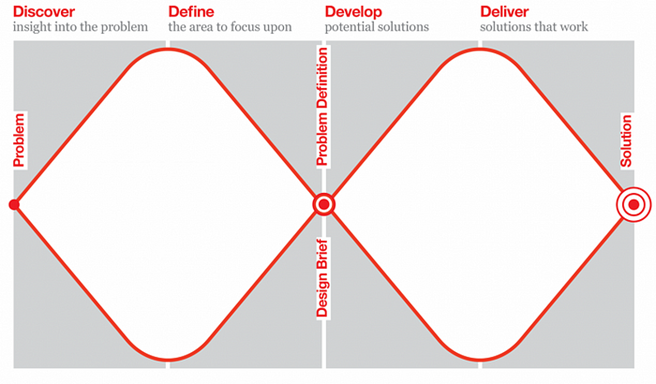
\includegraphics[width=0.8\linewidth]{image.png}
    \caption{Design Council's Double Diamond Process for User Centric and Interaction Design}
    \label{fig:Design Council's Double Diamond}
\end{figure}

\subsection{User Personas}
\begin{figure}[H]
    \centering
    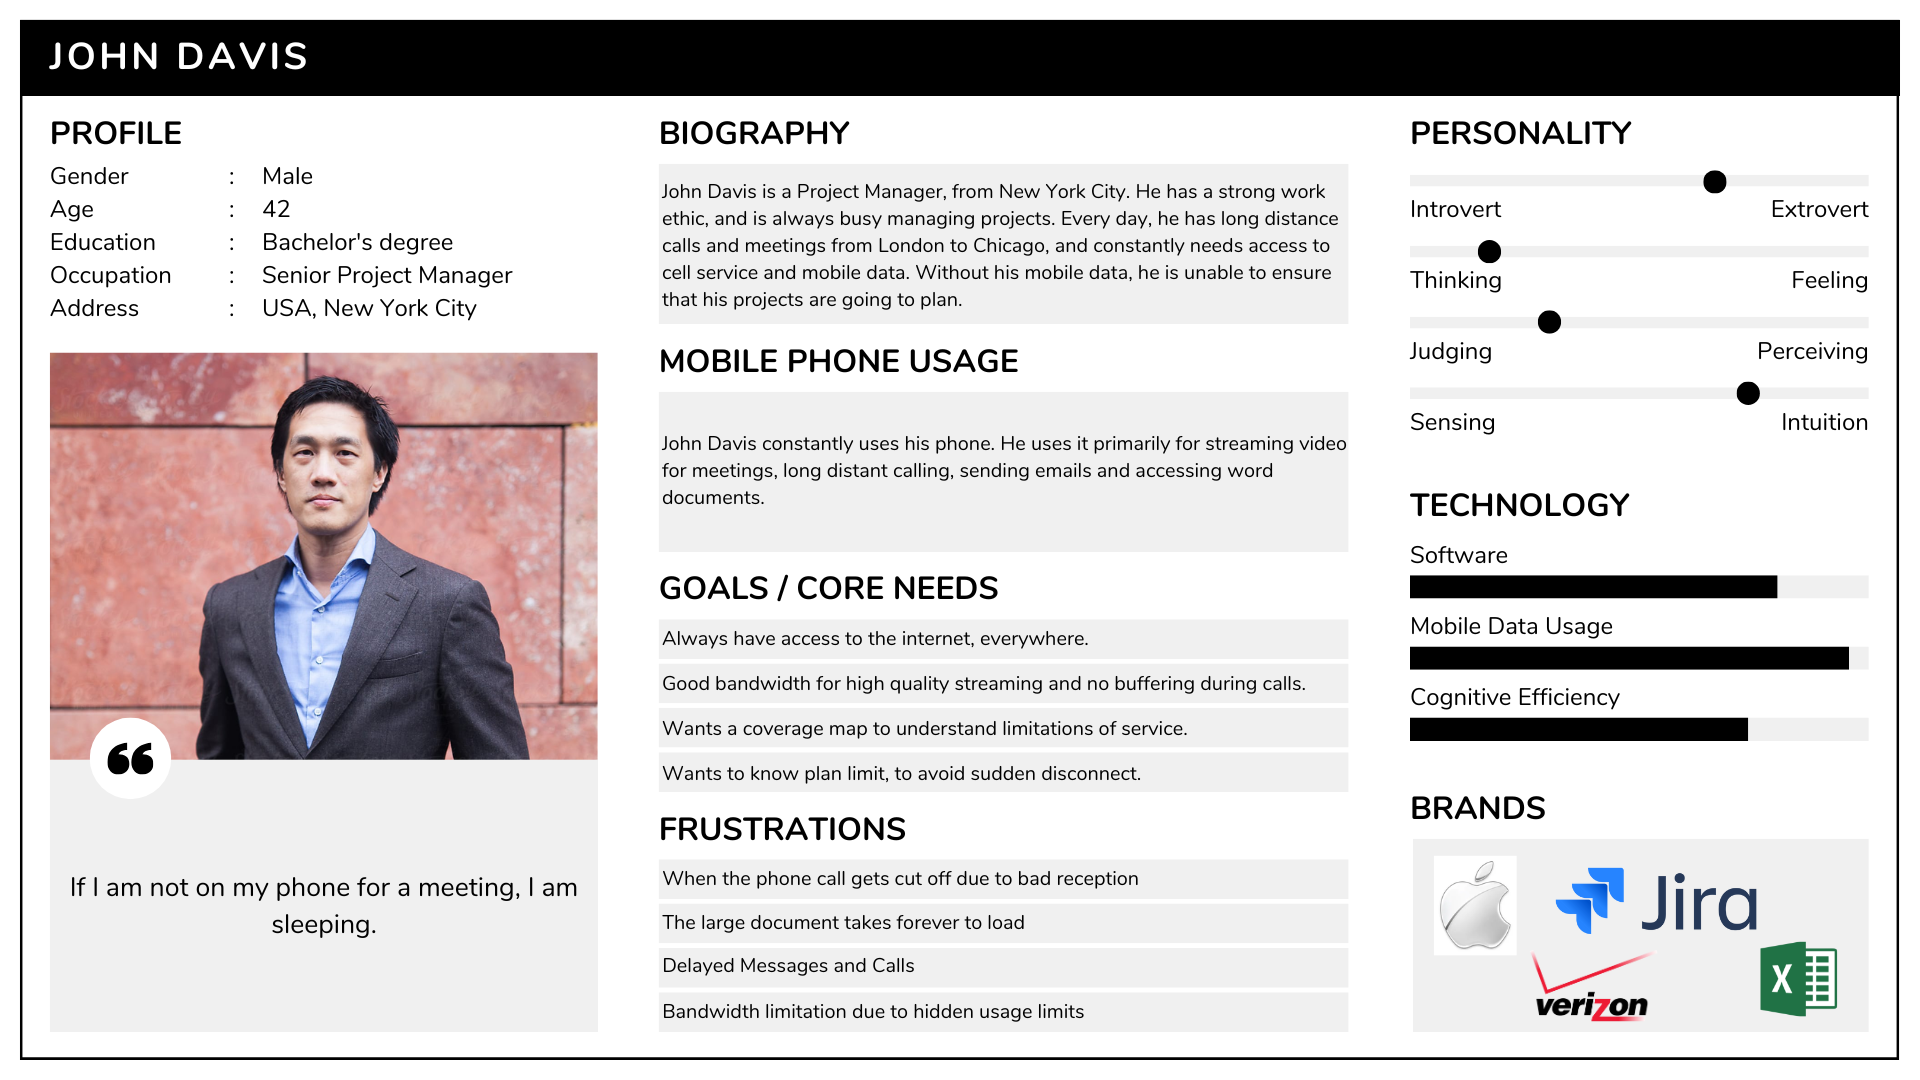
\includegraphics[width=1\linewidth]{persona_johndavis.png}
    \caption{User Persona relating to a need of constant data access}
    \label{fig:user persona 1}
\end{figure}

\begin{figure}[H]
    \centering
    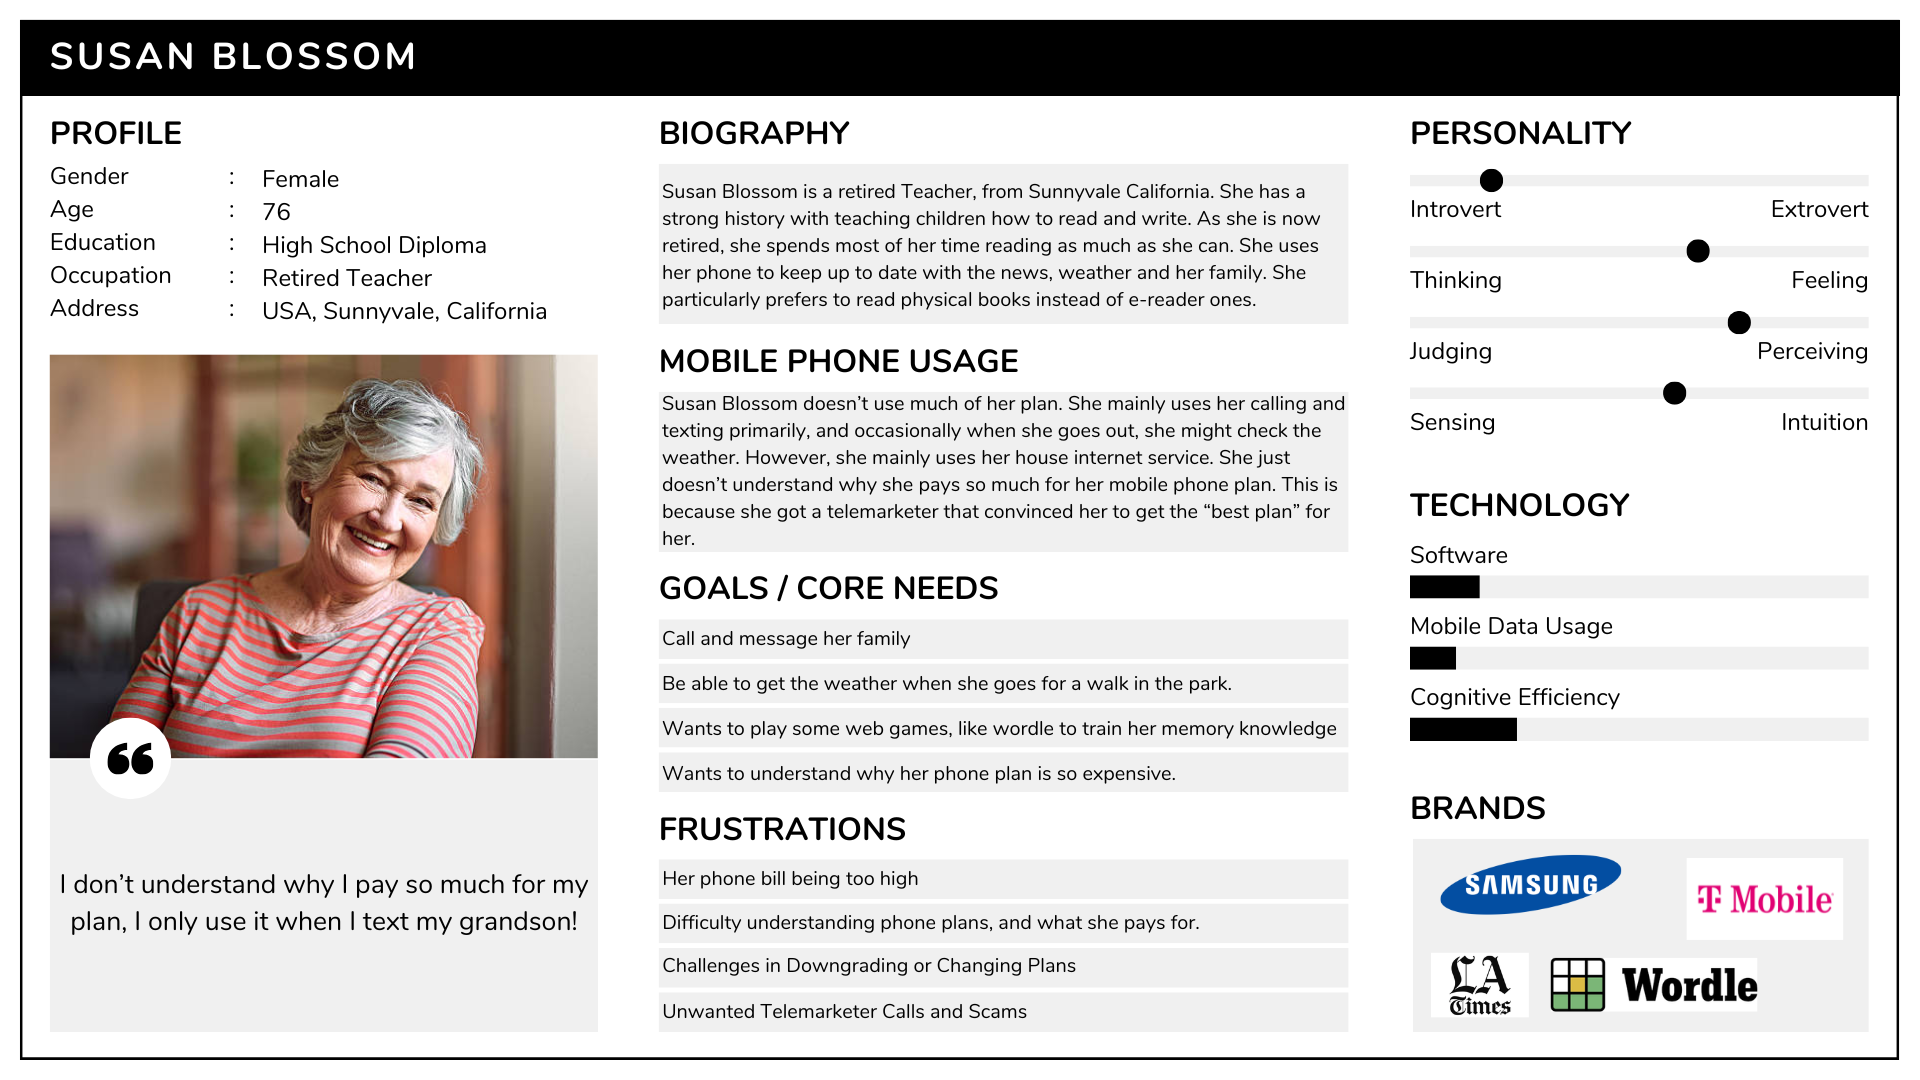
\includegraphics[width=1\linewidth]{persona_susanblossom.png}
    \caption{User Persona relating to a need of a better understanding of phone plans}
    \label{fig:user persona 2}
\end{figure}

\begin{figure}[H]
    \centering
    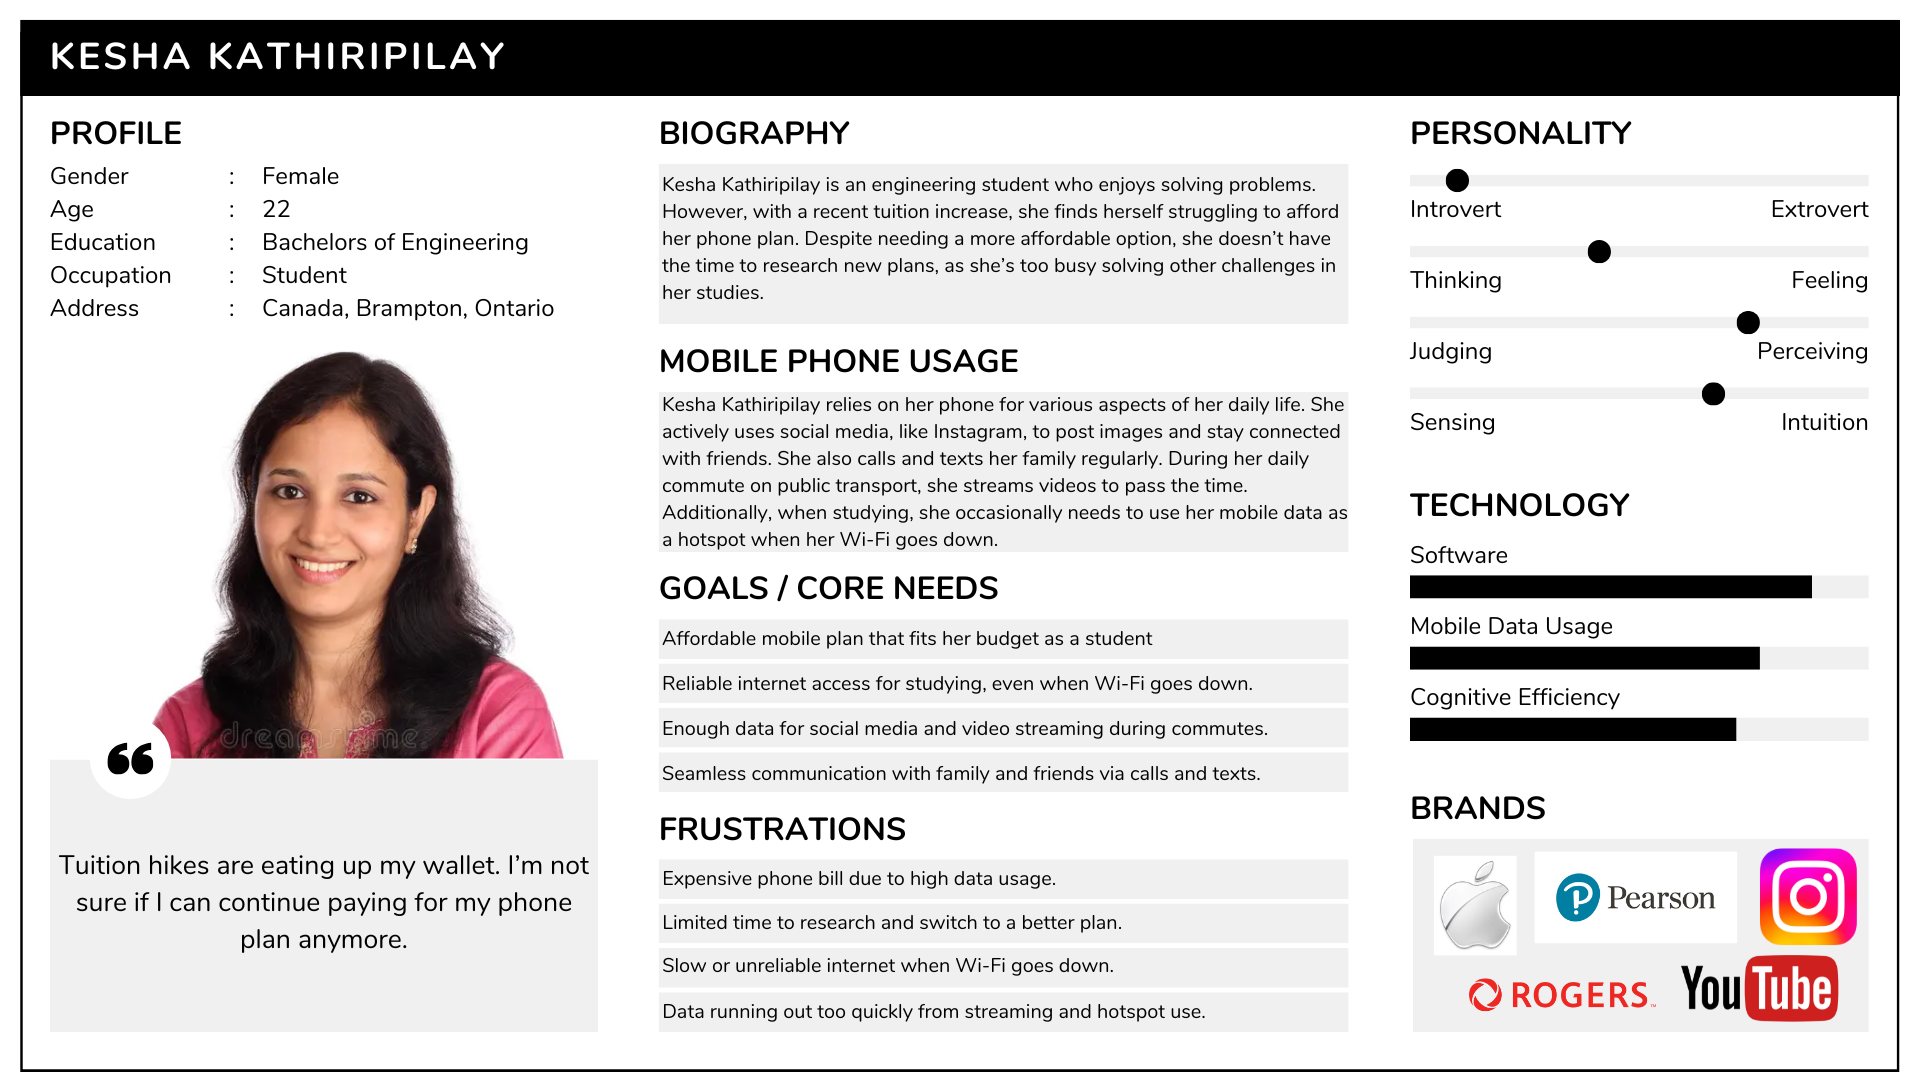
\includegraphics[width=1\linewidth]{persona_keshakath.png}
    \caption{User Persona relating to a need of a more affordable plan}
    \label{fig:user persona 3}
\end{figure}

\subsection{User Journey and Analysis}
\begin{figure}[H]
    \centering
    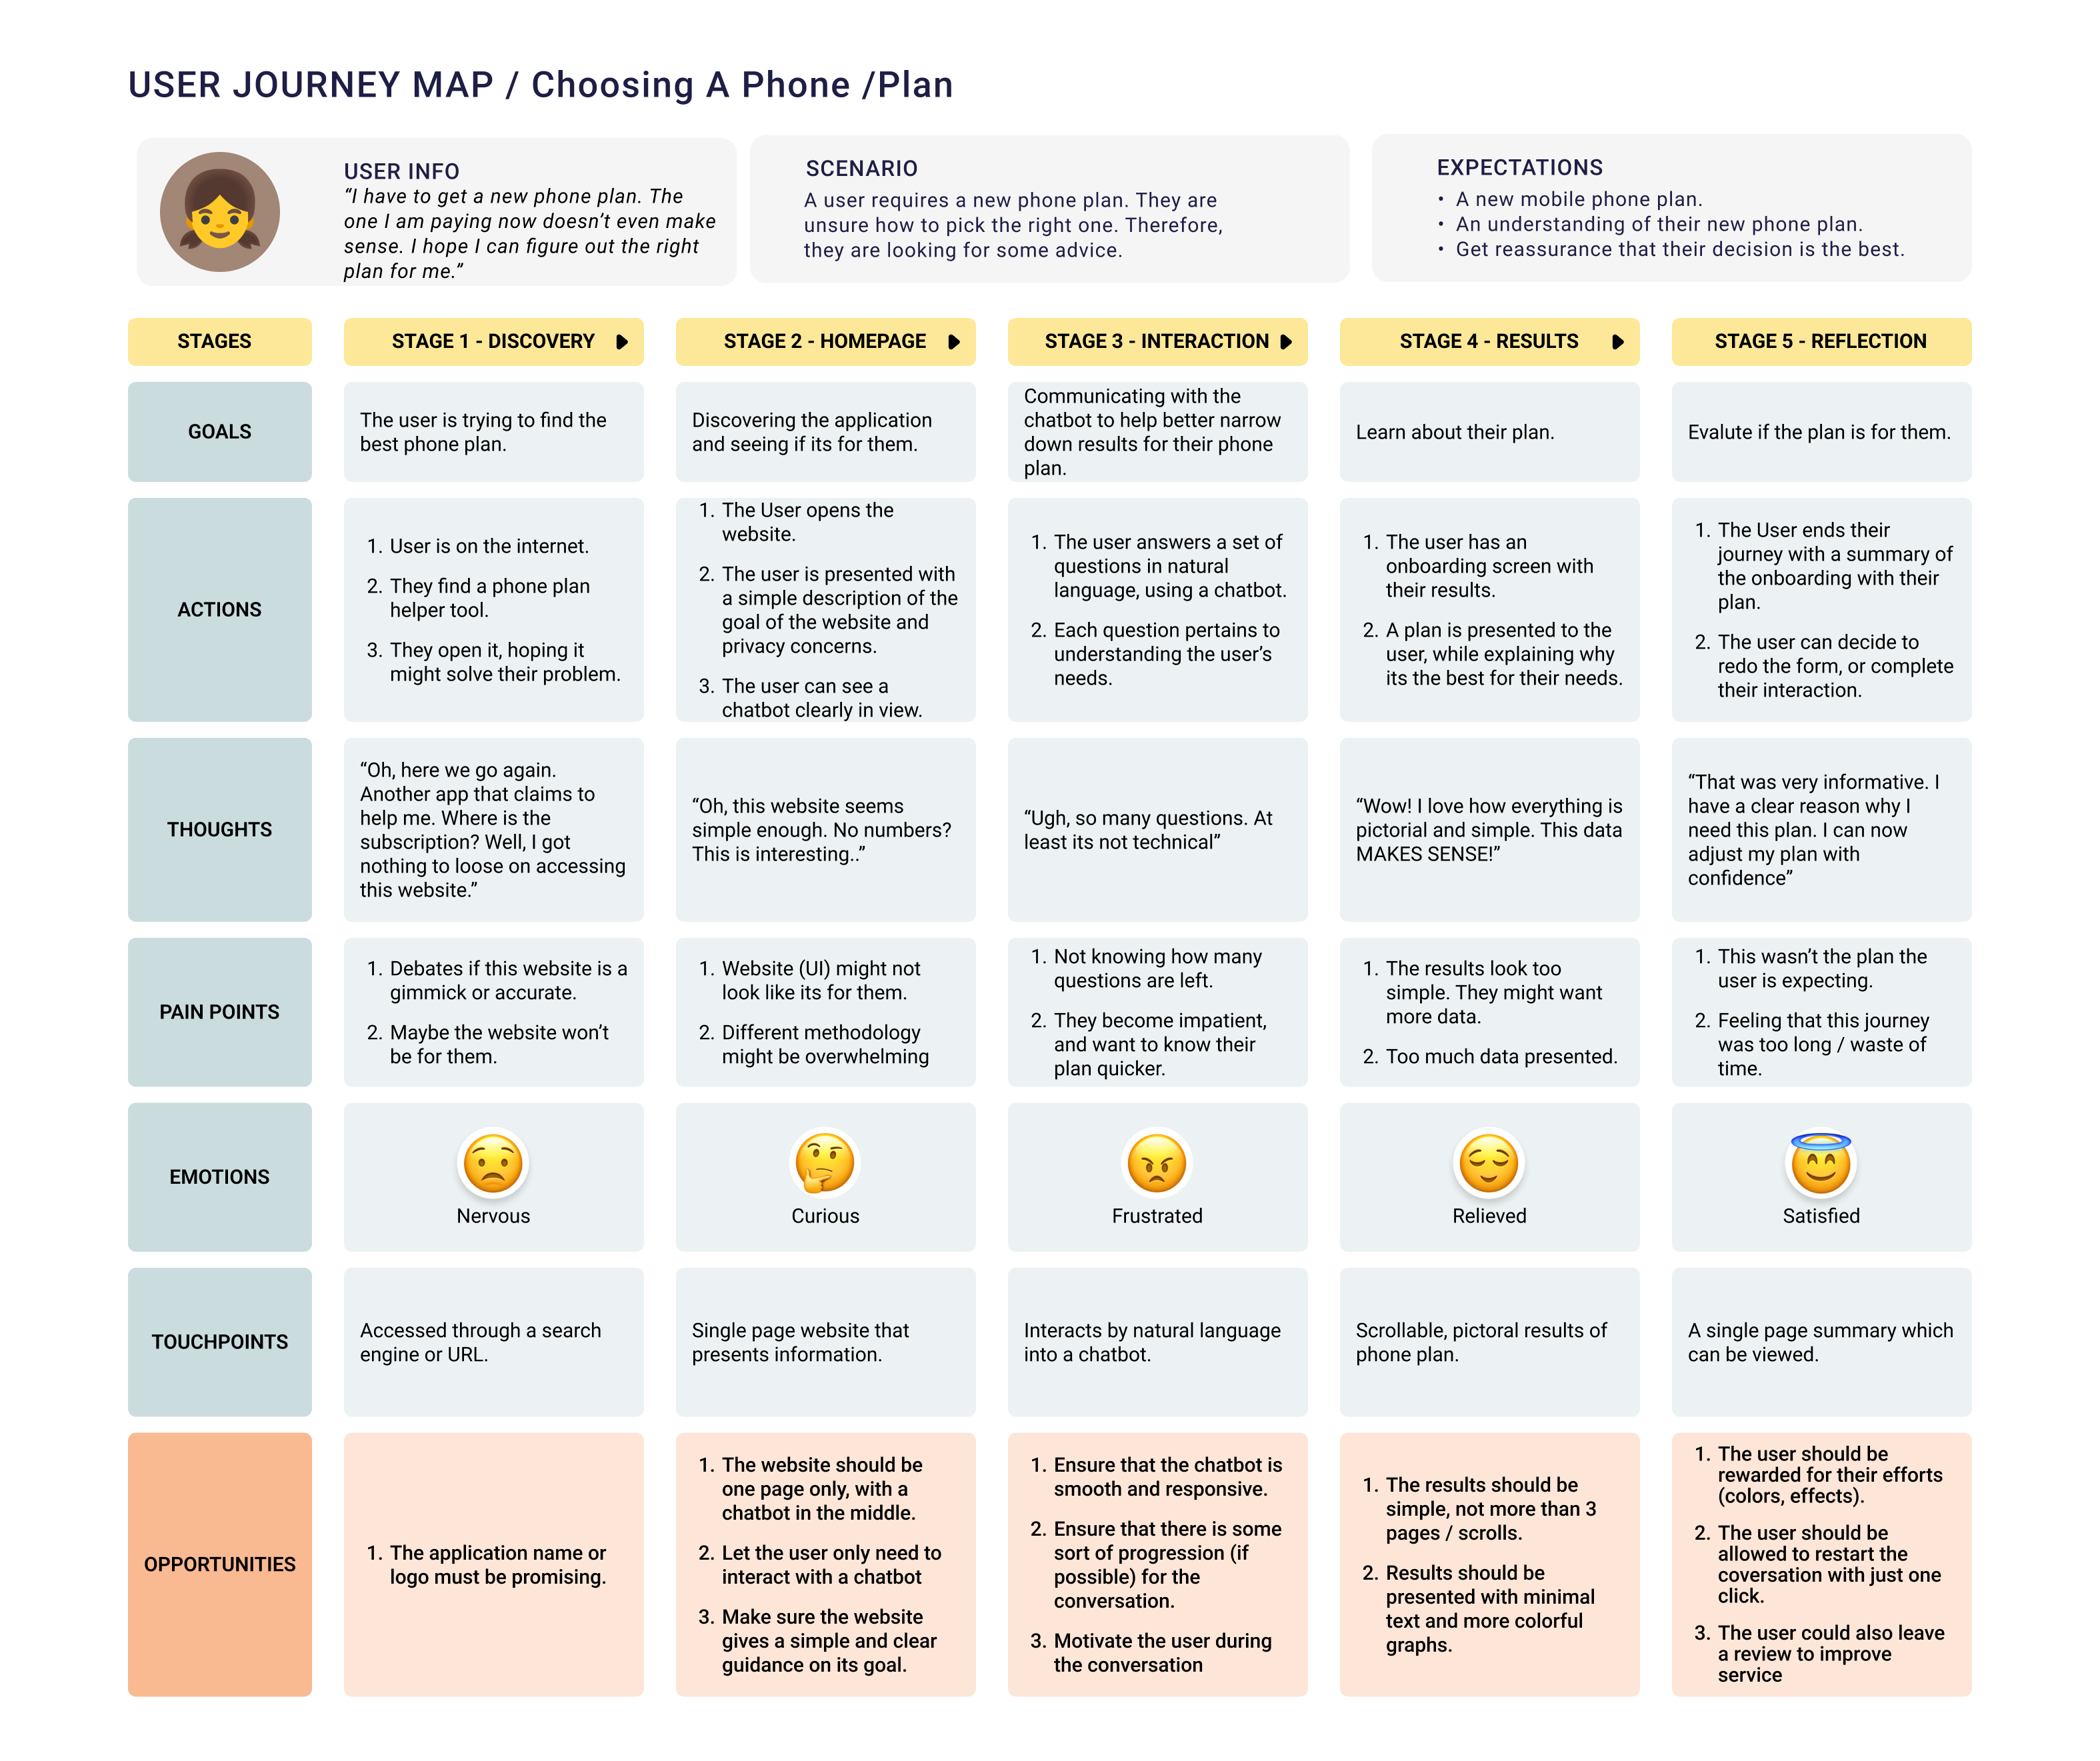
\includegraphics[width=1\linewidth]{User Journey Map_357research.jpg}
    \caption{User Journey of finding a Phone Plan}
    \label{fig:user journey}
\end{figure}

\begin{figure}[H]
    \centering
    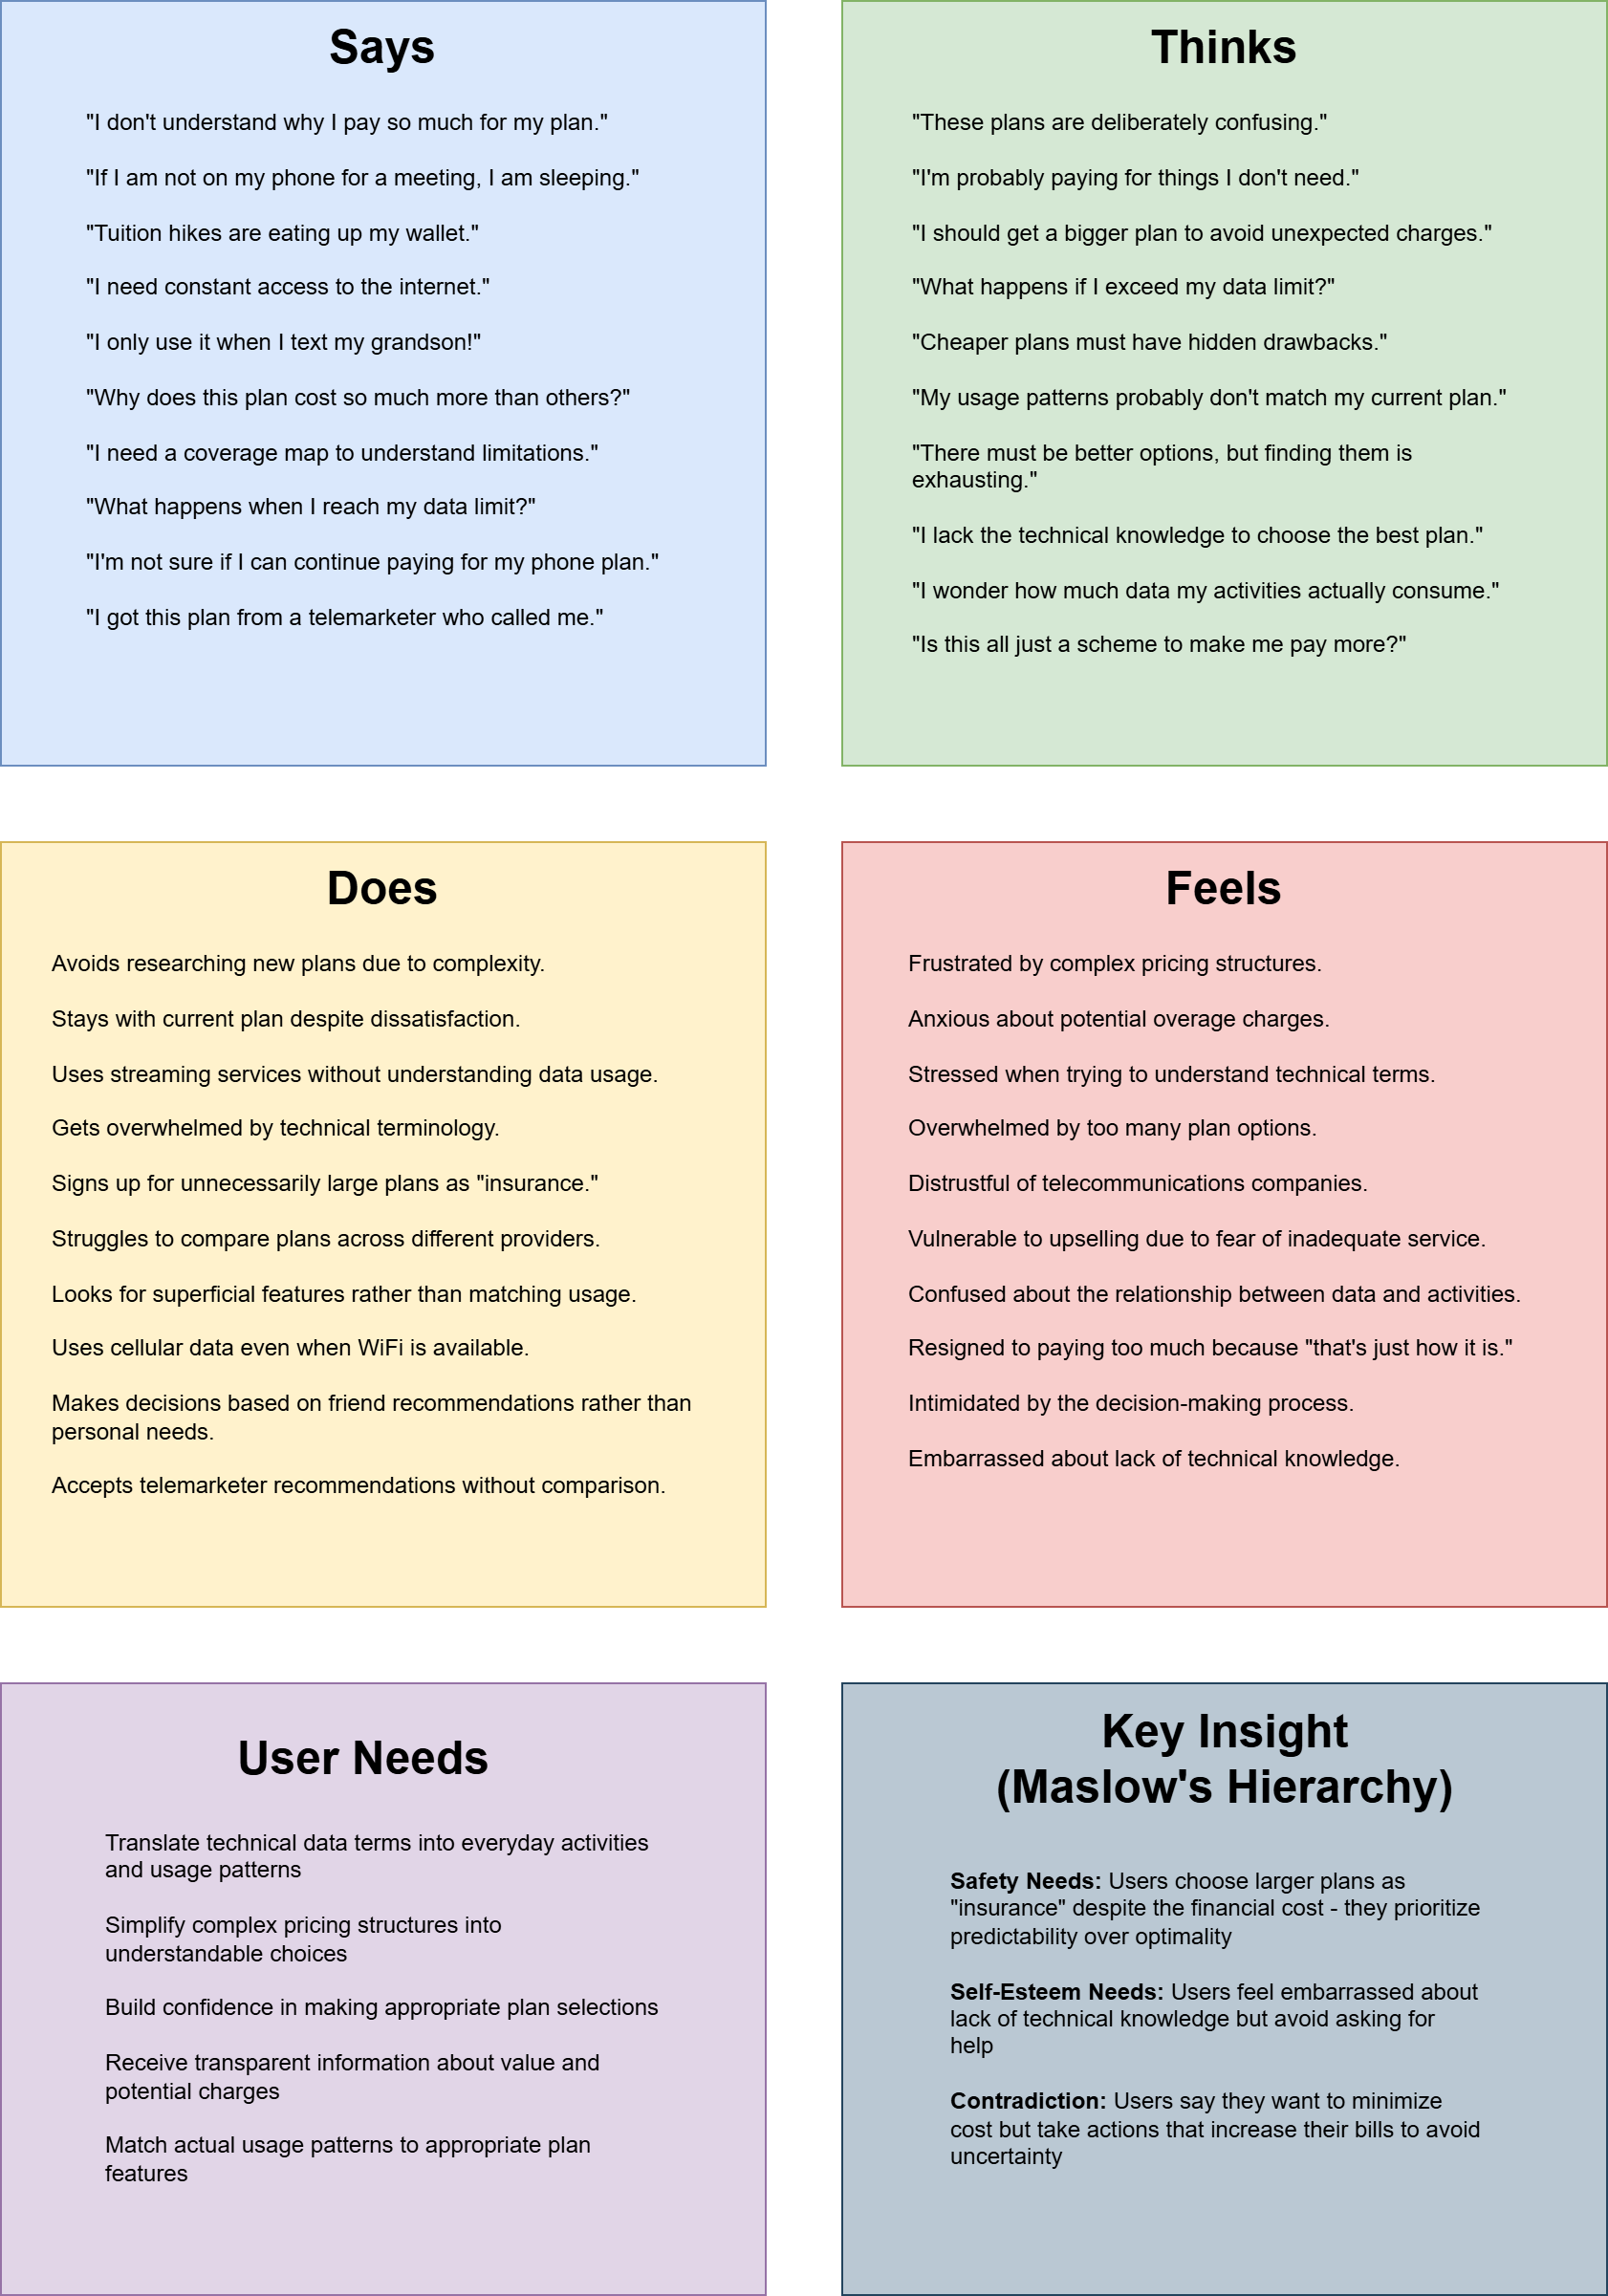
\includegraphics[width=1\linewidth]{EmpathyMap.png}
    \caption{Empathy map using Maslow's Hierarchy}
    \label{fig:empathy map}
\end{figure}

\begin{figure}[H]
    \centering
    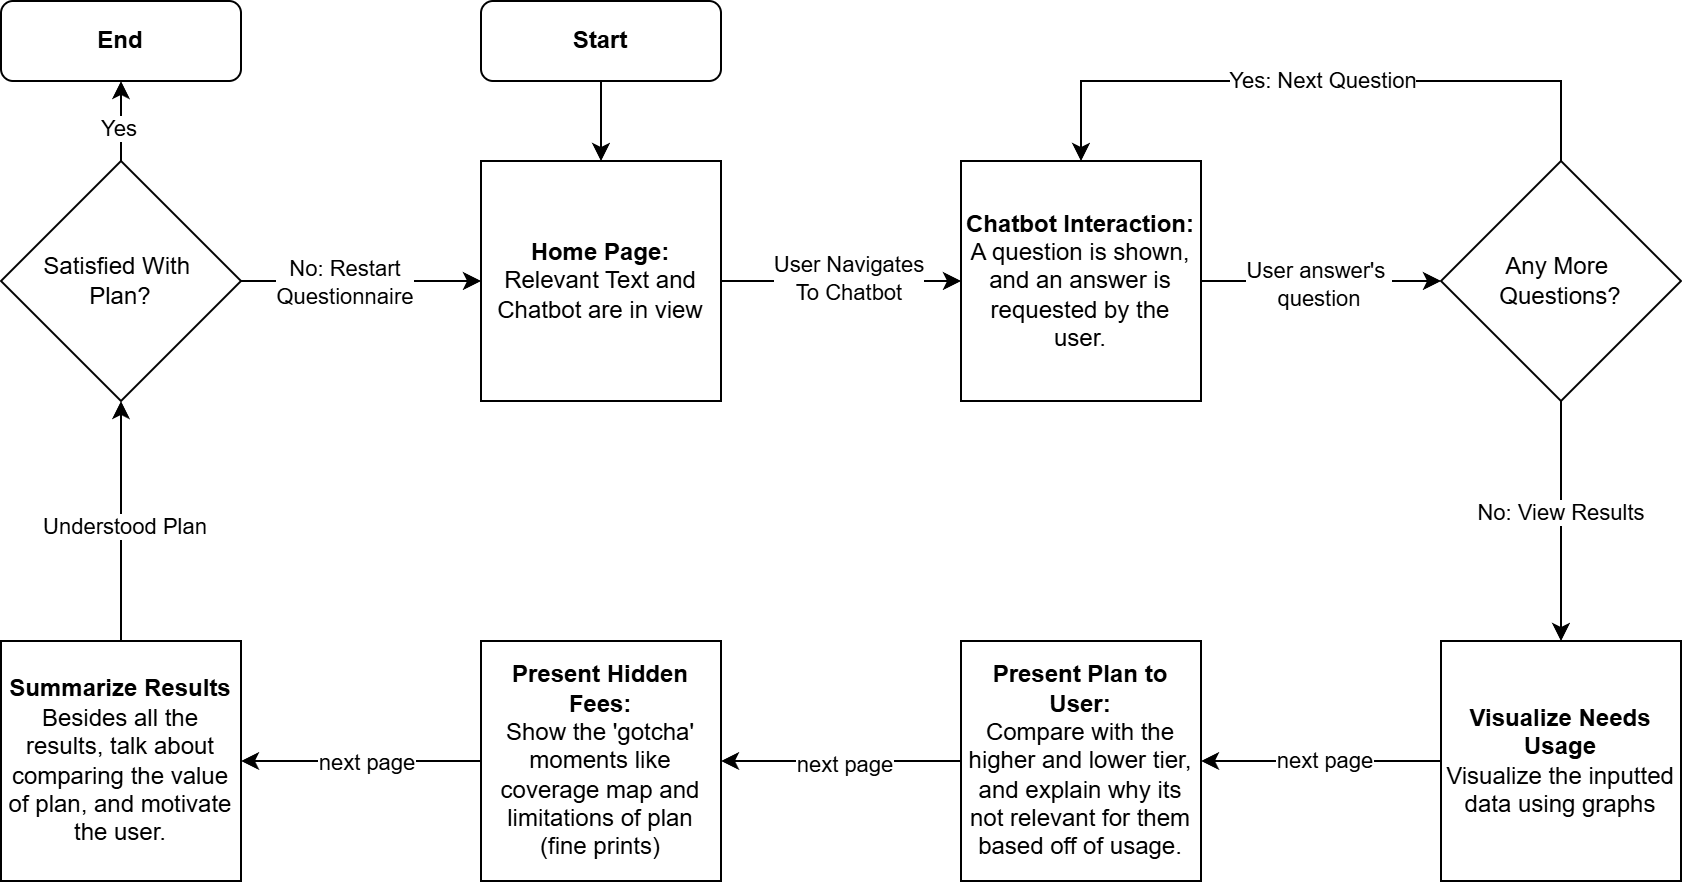
\includegraphics[width=1\linewidth]{FlowChart_357.png}
    \caption{User Flow Diagram of interacting with a Chatbot}
    \label{fig:user flow}
\end{figure}

\subsection{Scenario Maps}
\begin{figure}[H]
    \centering
    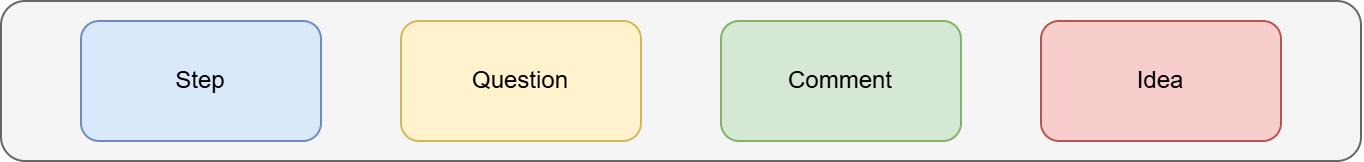
\includegraphics[width=1\linewidth]{ScenarioMap_Legend.drawio.png}
    \caption{Scenario Map Legend}
    \label{fig:scenario-map-legend}
\end{figure}

\begin{figure}[H]
    \centering
    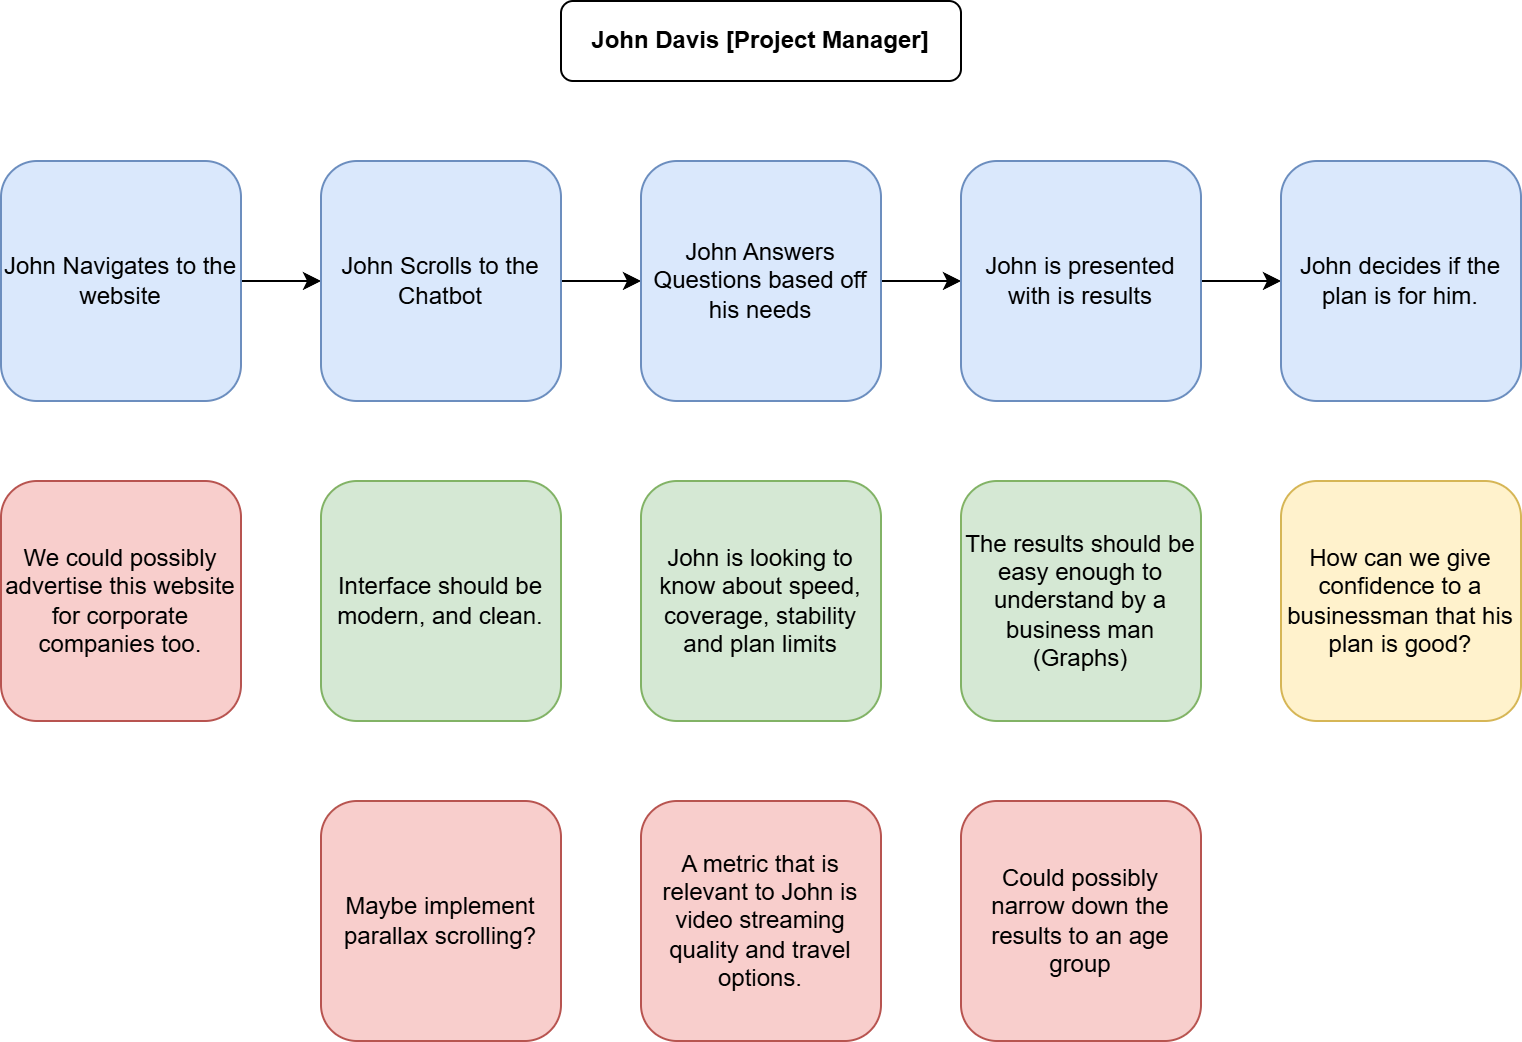
\includegraphics[width=1\linewidth]{ScenarioMap_John.drawio.png}
    \caption{Scenario map for John Davis}
    \label{fig:scenario-map-John}
\end{figure}

\begin{figure}[H]
    \centering
    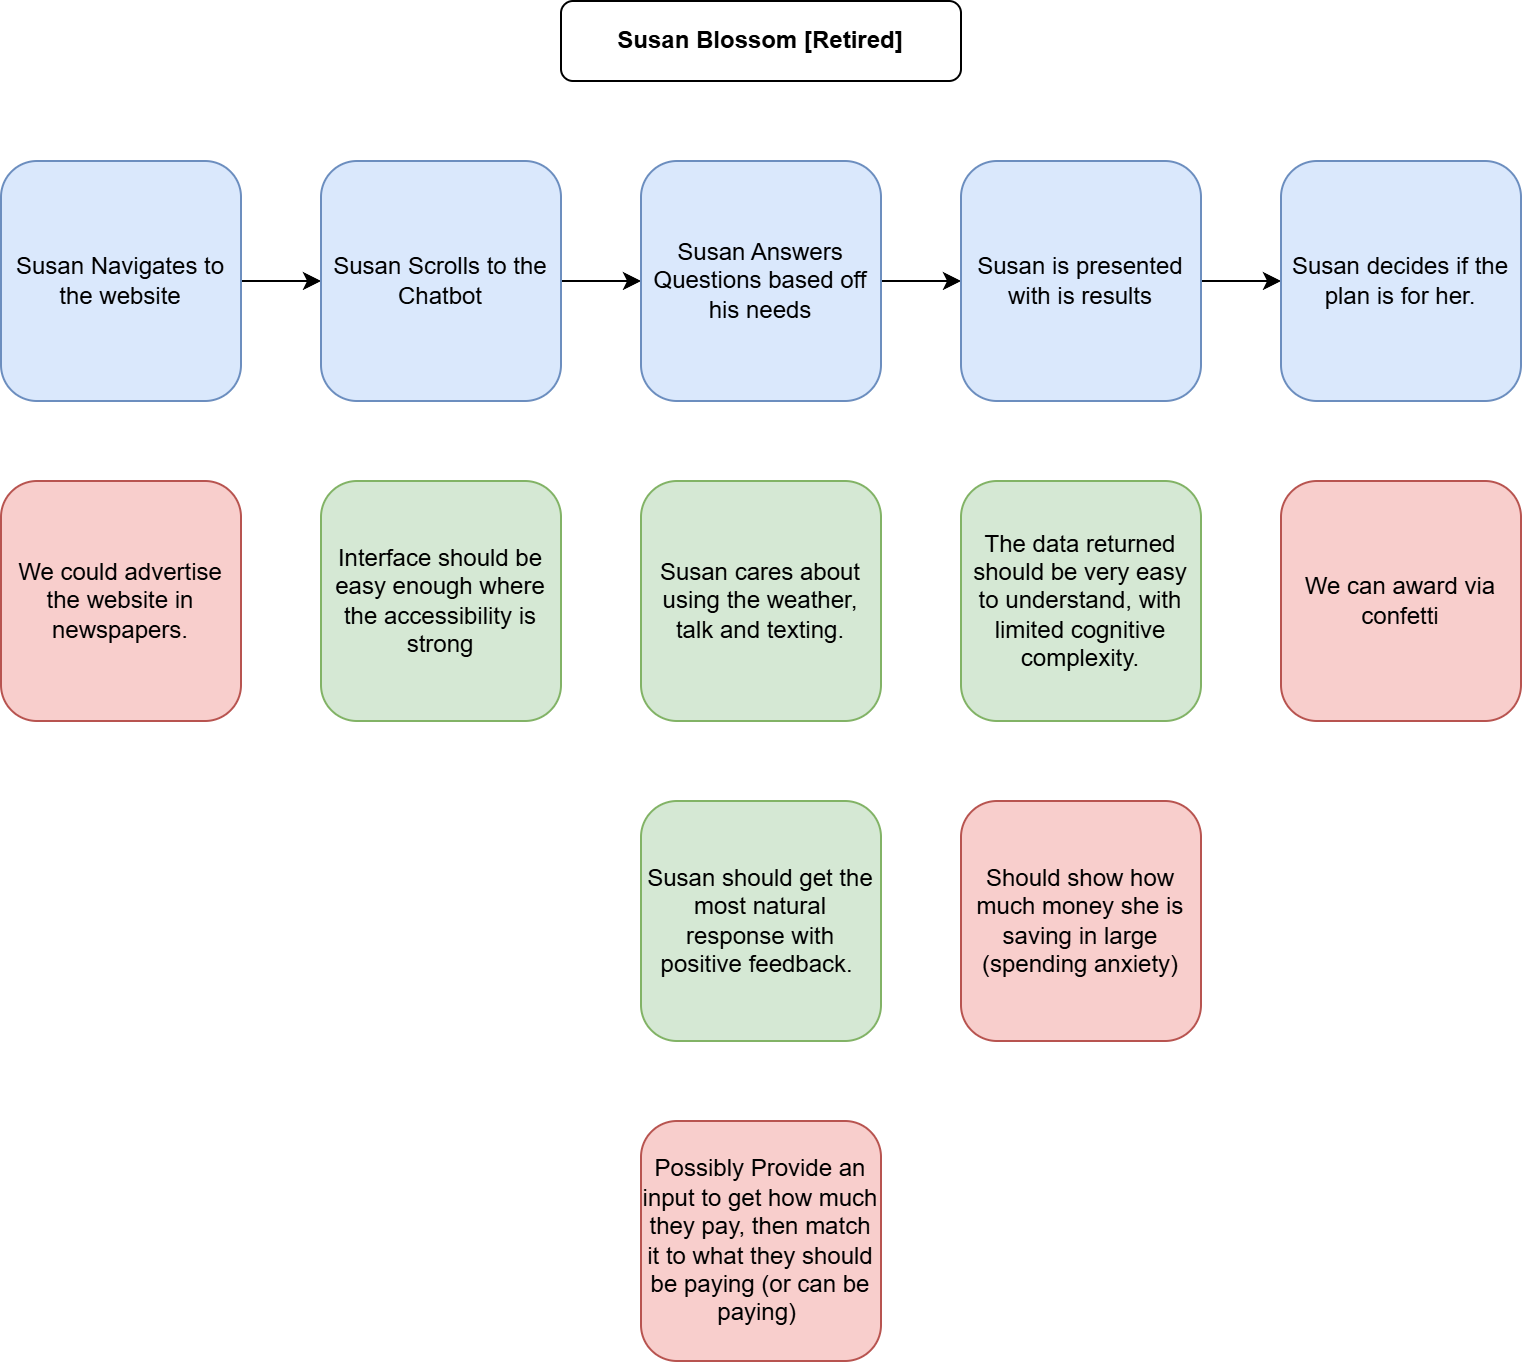
\includegraphics[width=1\linewidth]{ScenarioMap_Susan.drawio.png}
    \caption{Scenario map for Susan Blossom}
    \label{fig:scenario-map-Susan}
\end{figure}

\begin{figure}[H]
    \centering
    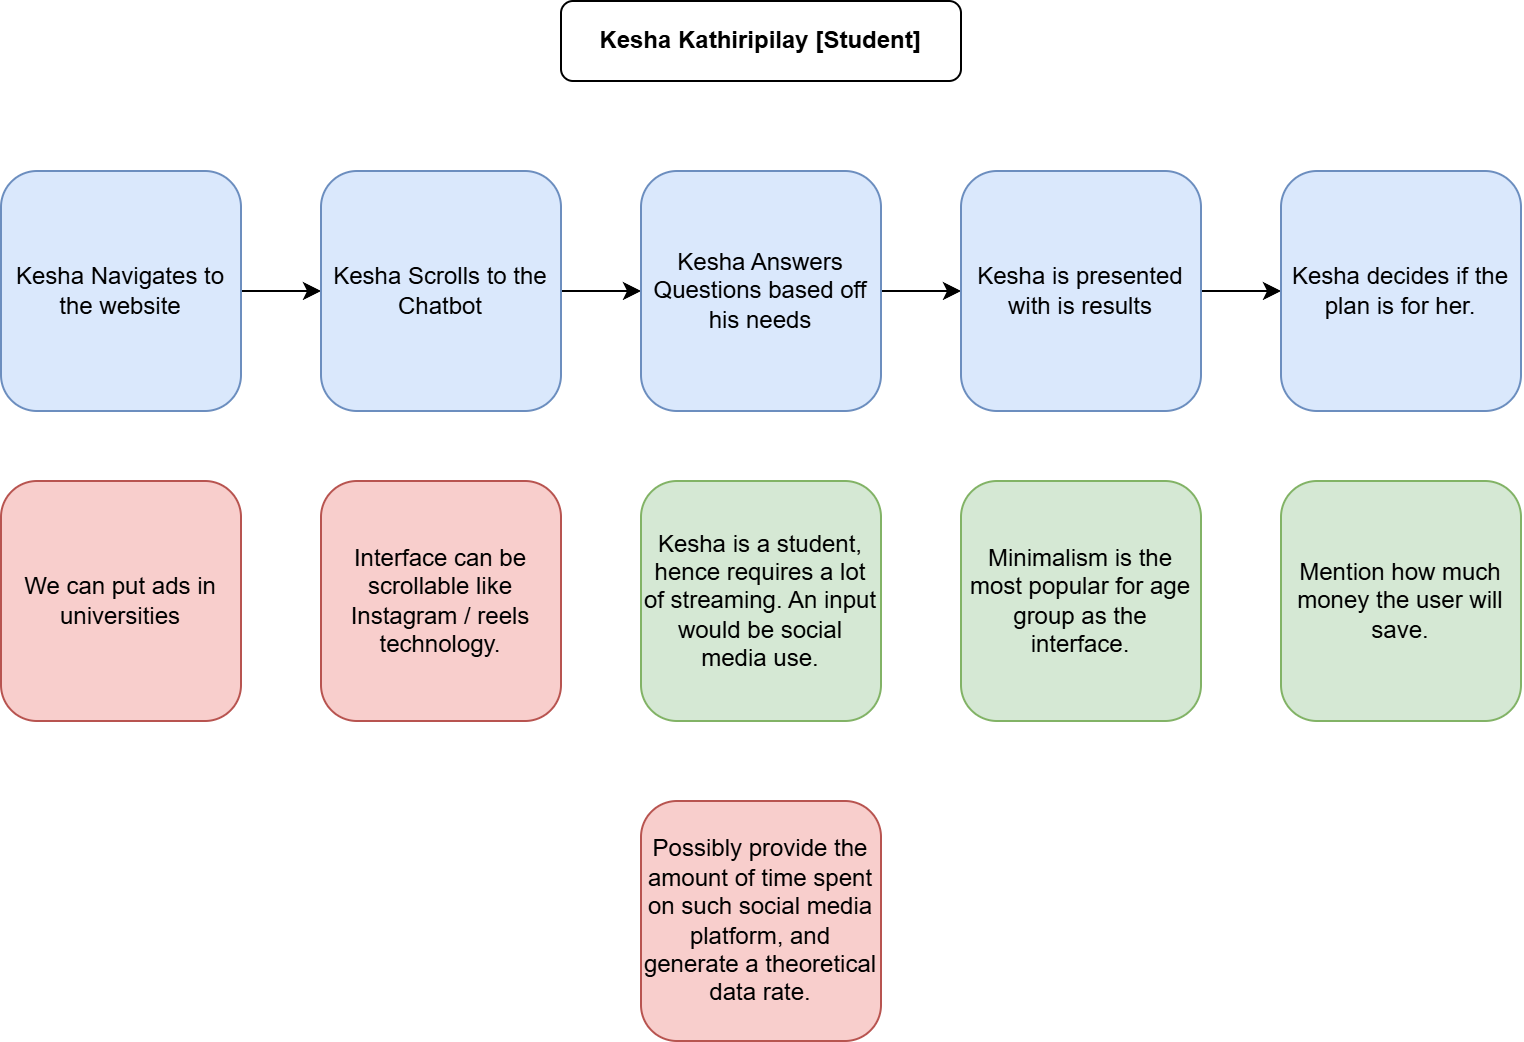
\includegraphics[width=1\linewidth]{ScenarioMap.Kesha-drawio.png}
    \caption{Scenario map for Kesha Kathiripilay}
    \label{fig:scenario-map-Kesha}
\end{figure}

\subsection{System Solution}
\begin{figure}[H]
    \centering
    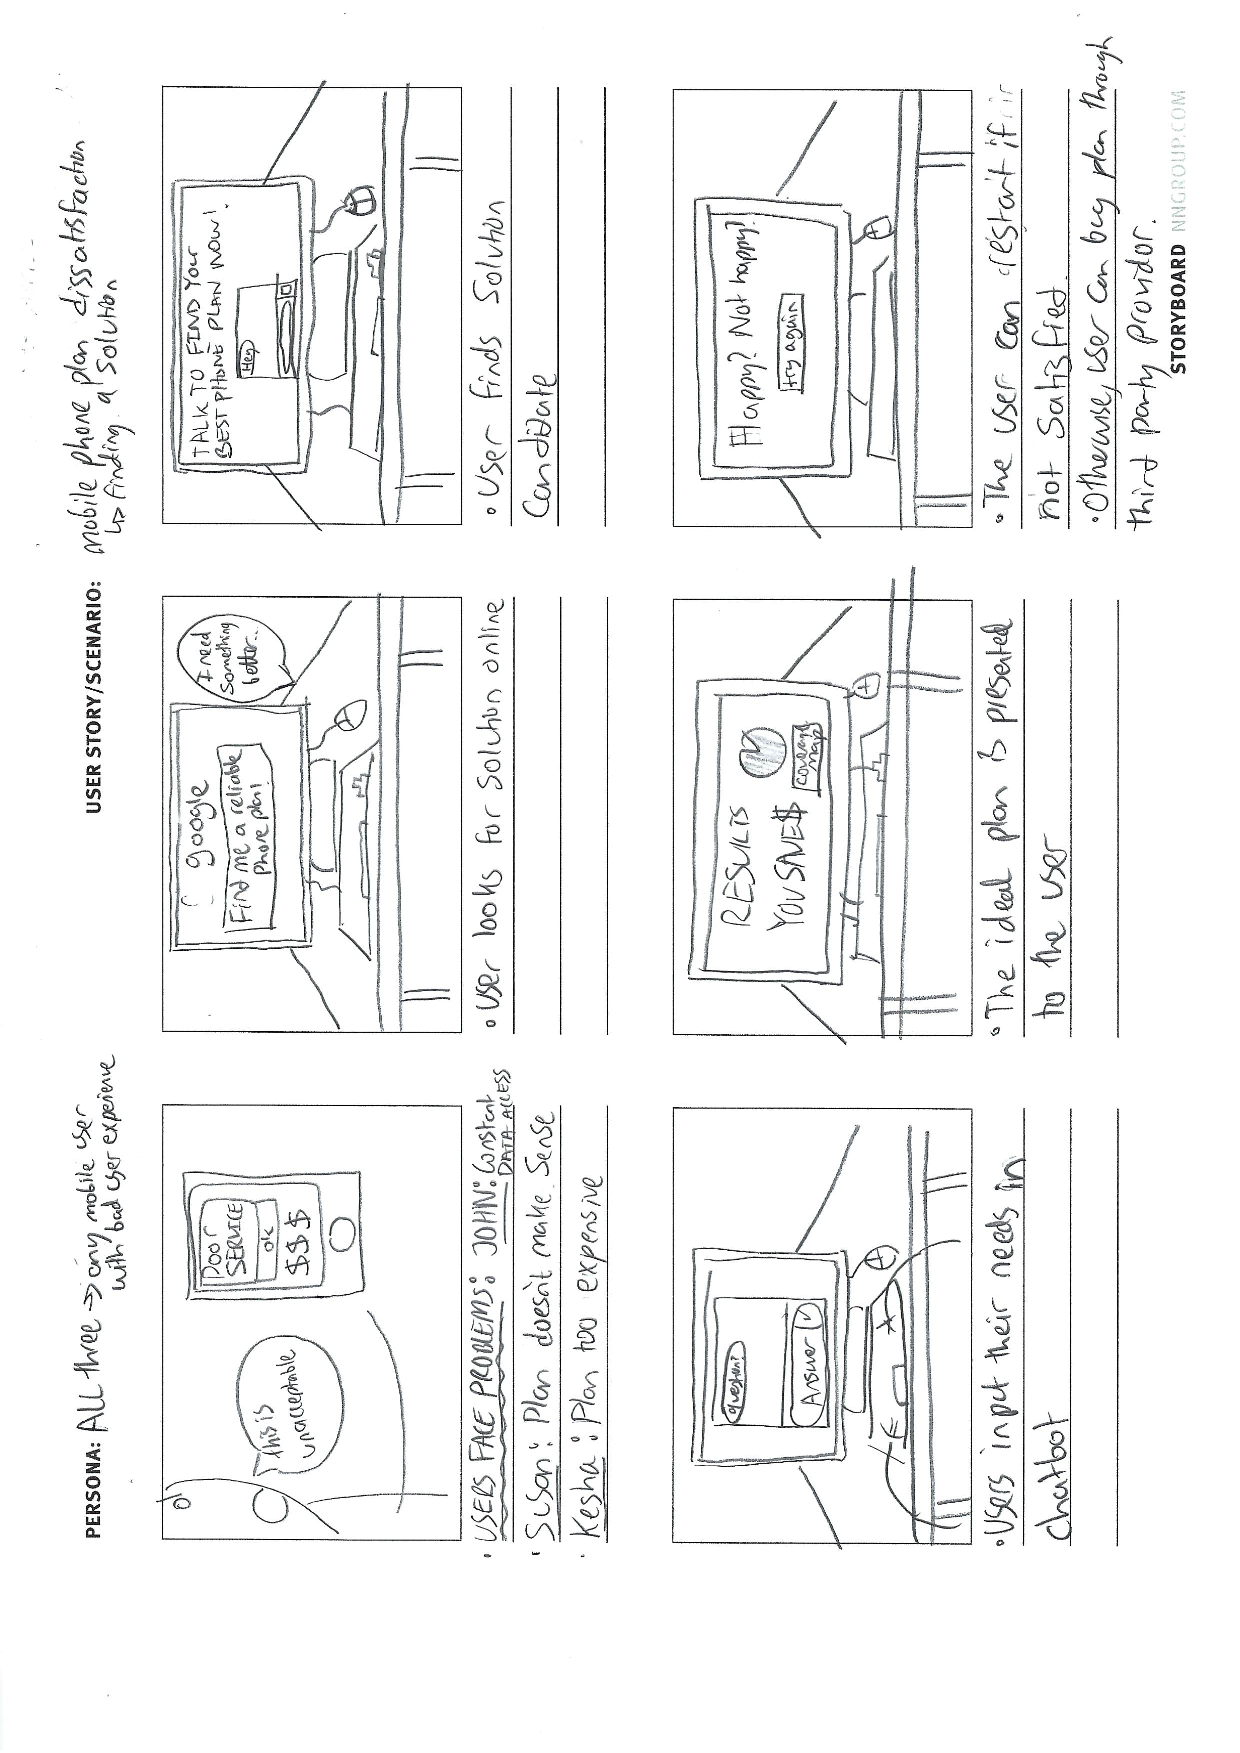
\includegraphics[width=1\linewidth]{storyboard.pdf}
    \caption{User Storyboard}
    \label{fig:story-board}
\end{figure}

\begin{figure}[H]
    \centering
    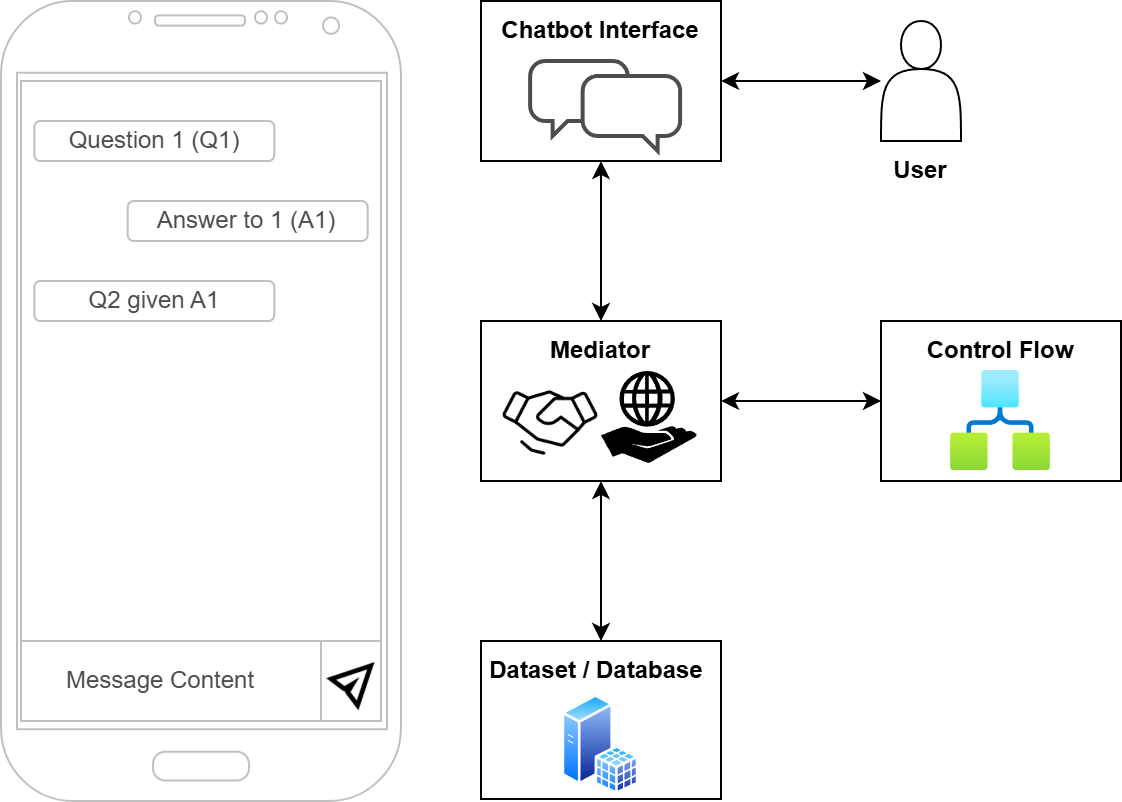
\includegraphics[width=1\linewidth]{Wireframe_Architecture.drawio.png}
    \caption{System Variables - Architecture of Problem}
    \label{fig:system-architecture}
\end{figure}
Appendix B: Original User Personas Descriptions
\subsection{John Davis}
A user with a need for constant data access. Key characteristics include professional requirements, usage habits, and pain points related to mobile data consumption.

\subsection{Susan Blossom}
A user seeking better understanding of phone plans. Key characteristics include her background, current challenges with technical terms, and desired outcomes from selecting a phone plan.

\subsection{Kesha Kathiripilay}
A user looking for a more affordable plan. Key characteristics include budget constraints, current usage patterns, and priorities when selecting a mobile phone plan.

\end{document}
